\noindent

This chapter presents the experimental validation of the proposed Modbus TCP threat monitoring framework. The objective of the evaluation is to verify whether the Suricata-based deep packet inspection rules can detect different types of Modbus TCP attack behaviors, and whether Graylog can support centralized alert management, event correlation, visualization, and standard-aligned traceability.

Although the framework proposed in Chapter 4 is organized into three logical layers, the experimental testbed was implemented using two virtual machines. The three layers represent logical functional separation rather than a strict one-to-one mapping to virtual or physical machines. In the implementation, the Attack Simulation Layer was deployed on an independent Kali Linux virtual machine, while the OT Simulation Layer and the Security Monitoring Layer were deployed on the same Ubuntu virtual machine

Five attack scenarios were implemented according to the detection rules proposed in Chapter 4, including reconnaissance scanning, Modbus protocol fuzzing, unauthorized modification, critical command injection, and denial-of-service flooding. Each scenario corresponds to a specific stage of the ICS Cyber Kill Chain and a Foundational Requirement of ISA/IEC 62443-3-3.

\section{Experimental Environment}
The experimental environment was established to validate the proposed Modbus TCP threat monitoring framework. The testbed emulates a simplified industrial control network in which attack traffic is generated toward a simulated Modbus TCP PLC/Slave device. The monitoring system inspects the traffic, detects suspicious Modbus TCP behaviors, and forwards security events to a centralized SIEM platform for visualization, alerting, and correlation analysis.

The experiment focuses on evaluating whether the proposed framework can detect representative Modbus TCP threat behaviors and present the corresponding alerts in a structured and traceable manner. The evaluated scenarios include reconnaissance scanning, protocol fuzzing, unauthorized write operations, diagnostic command injection, and denial-of-service flooding. These scenarios were selected to represent different stages of Modbus TCP attack behavior and to verify the detection capability of the proposed rules.

The overall experimental design follows the three logical layers proposed in Chapter 4: the Attack Simulation Layer, the OT Simulation Layer, and the Security Monitoring Layer. These layers are used to describe the functional roles of the framework. The detailed mapping between the logical layers and the actual virtual machine deployment is described in Section 5.1.1.

\subsection{Hardware and Virtualization Environment}
The experimental testbed was implemented in a virtualized environment hosted on a physical machine. The host machine is equipped with an Intel(R) Core(TM) i5-4440 CPU @ 3.10GHz, 32 GB of memory (8 GB 1600MHz × 4), and 1 TB of storage, operating on Windows 10 Professional 21H1. Within this virtualized environment, two virtual machines were deployed. Although the proposed framework consists of three logical layers, these layers represent functional separation rather than a strict one-to-one mapping to physical or virtual machines. Therefore, the Attack Simulation Layer was deployed on VM1, while the OT Simulation Layer and the Security Monitoring Layer were deployed on VM2.

VM1 was configured as the attack host using Kali Linux 2025.04. It was responsible for generating attack traffic for the experimental scenarios, including reconnaissance scanning, protocol fuzzing, unauthorized Modbus write operations, diagnostic command injection, and TCP SYN flooding. VM2 was configured using Ubuntu 22.04.5 LTS and hosted both the Modbus TCP simulation environment and the monitoring components. ModbusPal and Suricata were executed directly on VM2, while the Graylog SIEM stack, including Graylog, OpenSearch, and MongoDB, was deployed using Docker containers. Figure~\ref{fig:Figure_5.1.jpg} illustrates the mapping between the logical layers of the proposed framework and the actual virtual machine deployment.

\begin{figure}[htbp]
\centering
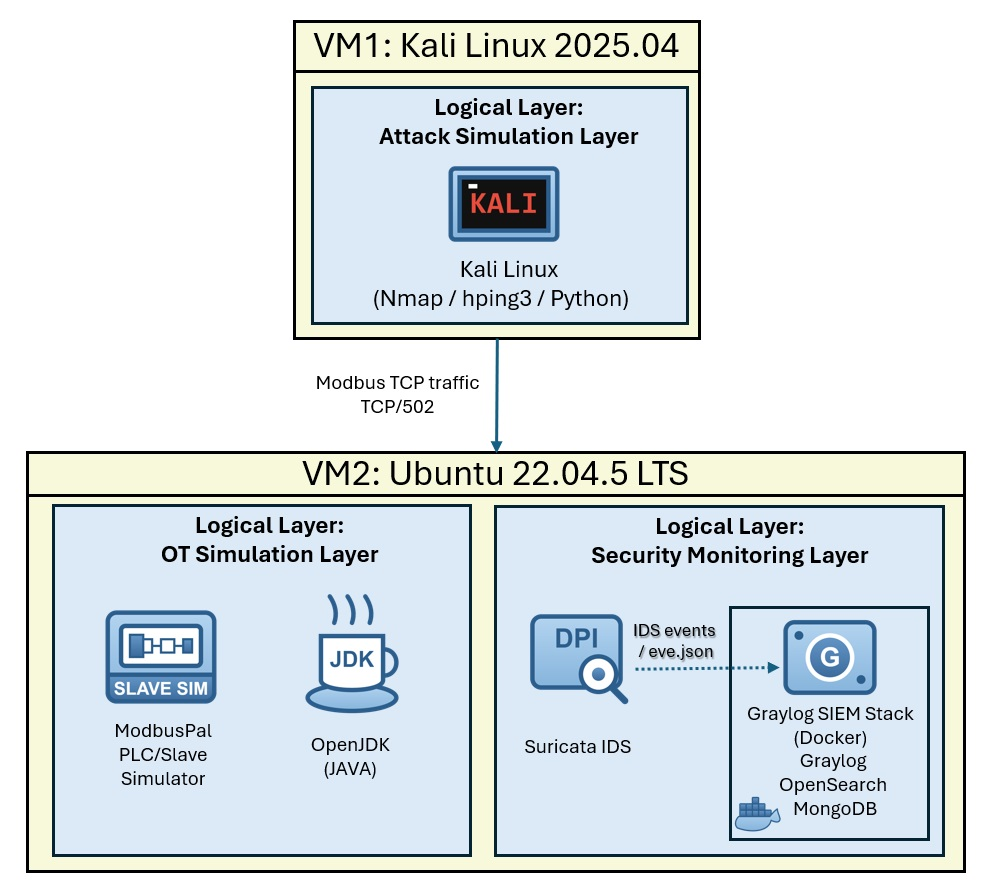
\includegraphics[width=13.5cm]{figure/Figure_5.1.jpg}
\caption{Mapping of Logical Layers to Virtual Machine Deployment} \label{fig:Figure_5.1.jpg}
\end{figure}

\newpage

As shown in Figure~\ref{fig:Figure_5.1.jpg}, Modbus TCP traffic was generated from VM1 to VM2 through TCP port 502. Suricata monitored the Modbus TCP traffic on VM2 and forwarded IDS events in eve.json format to the Graylog SIEM stack for further analysis and visualization.Table~\ref{tab:layer_vm_mapping} summarizes the mapping between the logical layers and the virtual machine deployment.

\begin{table}[htbp]
\caption{Mapping between Logical Layers and Virtual Machines}
\centering
\renewcommand{\arraystretch}{1.35}
\setlength{\tabcolsep}{6pt}
\resizebox{\linewidth}{!}{%
\begin{tabular}{|p{2.1cm}|p{3.6cm}|p{3.2cm}|p{5cm}|}
\hline
\textbf{Logical Layer} & \textbf{Implementation} & \textbf{Deployment} & \textbf{Main \newline Components} \\
\hline
Attack Simulation Layer & Independent \newline attack VM & VM1 & Kali Linux, Nmap, hping3, Python \\
\hline
OT \newline Simulation Layer & PLC/Slave \newline simulator & VM2 native & Ubuntu, ModbusPal, OpenJDK \\
\hline
Security Monitoring Layer & IDS and SIEM \newline monitoring services & VM2 native and Docker containers & Suricata, Docker, Graylog, OpenSearch, MongoDB \\
\hline
\end{tabular}%
}
\label{tab:layer_vm_mapping}
\end{table}

The Attack Simulation Layer was implemented as an independent attack VM. The OT Simulation Layer and the Security Monitoring Layer were both deployed on VM2 but remained logically separated by function. Table \ref{tab:vm_configuration} summarizes the virtual machine configuration used in the experiment.

\begin{table}[htbp]
\caption{Virtual Machine Configuration}
\centering
\renewcommand{\arraystretch}{1.35}
\setlength{\tabcolsep}{6pt}
\resizebox{\linewidth}{!}{%
\begin{tabular}{|p{1cm}|p{2.2cm}|p{2.8cm}|p{9.5cm}|}
\hline
\textbf{VM} & \textbf{Operating \newline System} & \textbf{vCPU/RAM} & \textbf{Role} \\
\hline
VM1 & Kali Linux & 2 Cores, 4 GB & Attack Simulation Layer \\
\hline
VM2 & Ubuntu & 4 Cores, 20 GB & OT Simulation Layer and Security Monitoring Layer \\
\hline
\end{tabular}%
}
\label{tab:vm_configuration}
\end{table}

VM1 was used to generate attack traffic, while VM2 integrated the Modbus TCP simulation, IDS monitoring, and SIEM analysis functions.

\newpage

\subsection{Software Tools and Versions}
This section focuses on the main software tools and services used for attack
simulation, OT simulation, and security monitoring. The operating systems and
kernel versions of the virtual machines were described in the previous subsection;
therefore, they are not repeated in the software configuration table. Although the
OT Simulation Layer and the Security Monitoring Layer were both deployed on
VM2, they remained logically separated according to their functions.

As shown in Table \ref{tab:software_configuration}, Nmap, hping3, and Python were used in the Attack
Simulation Layer to generate different types of Modbus TCP attack traffic.
ModbusPal and OpenJDK were used in the OT Simulation Layer to emulate a
Modbus TCP PLC/Slave device. In the Security Monitoring Layer, Suricata was
deployed natively on VM2 as the IDS engine, while Graylog, OpenSearch, and
MongoDB were deployed as Docker containers to provide centralized log
management, indexing, search, and alert visualization.

\begin{table}[htbp]
\caption{Software Configuration by Logical Layer}
\centering
\renewcommand{\arraystretch}{1.35}
\setlength{\tabcolsep}{6pt}
\resizebox{\linewidth}{!}{%
\begin{tabular}{|p{3.8cm}|p{2.4cm}|p{2.4cm}|p{2.4cm}|p{6.2cm}|}
\hline
\textbf{Logical Layer} & \textbf{Component} & \textbf{Version} & \textbf{Deployment} & \textbf{Role} \\
\hline
Attack Simulation Layer & Nmap & 7.95 & VM1 & Modbus service discovery and reconnaissance scanning \\
\hline
Attack Simulation Layer & hping3 & 3.0.0-alpha-2 & VM1 & DoS traffic generation \\
\hline
Attack Simulation Layer & Python & 3.13.9 & VM1 & Custom attack script execution \\
\hline
OT Simulation Layer & ModbusPal & 1.6c & VM2 native & Modbus TCP PLC/Slave simulator \\
\hline
OT Simulation Layer & OpenJDK & 11.0.30 & VM2 native & Java runtime environment for ModbusPal \\
\hline
OT Simulation Layer & pymodbus & 3.8.6 & VM2 native & Modbus TCP communication library \\
\hline
Security Monitoring Layer & Suricata & 7.0.x & VM2 native & IDS engine for Modbus TCP monitoring \\
\hline
Security Monitoring Layer & Docker & 29.1.3 & VM2 native & Container runtime for SIEM services \\
\hline
Security Monitoring Layer & Graylog & 5.2.12 & VM2 Docker container & SIEM platform \\
\hline
Security Monitoring Layer & OpenSearch & 2.12.0 & VM2 Docker container & Log indexing and search backend \\
\hline
Security Monitoring Layer & MongoDB & 5.0 & VM2 Docker container & Graylog metadata database \\
\hline
\end{tabular}%
}
\label{tab:software_configuration}
\end{table}

\newpage

\subsection{Experimental Testbed and Baseline Traffic Validation}
The experimental testbed was deployed in an isolated virtual network to emulate a simplified Modbus TCP-based industrial control system environment. As shown in Figure~\ref{fig:Figure_5.2.jpg}, the testbed consisted of two virtual machines connected to the same virtual network segment, 192.168.11.0/24. VM1 was used as the traffic generation and attack simulation host, while VM2 hosted the Modbus TCP PLC simulator, the Suricata intrusion detection system, and the Graylog SIEM stack.

\begin{figure}[htbp]
    \centering
    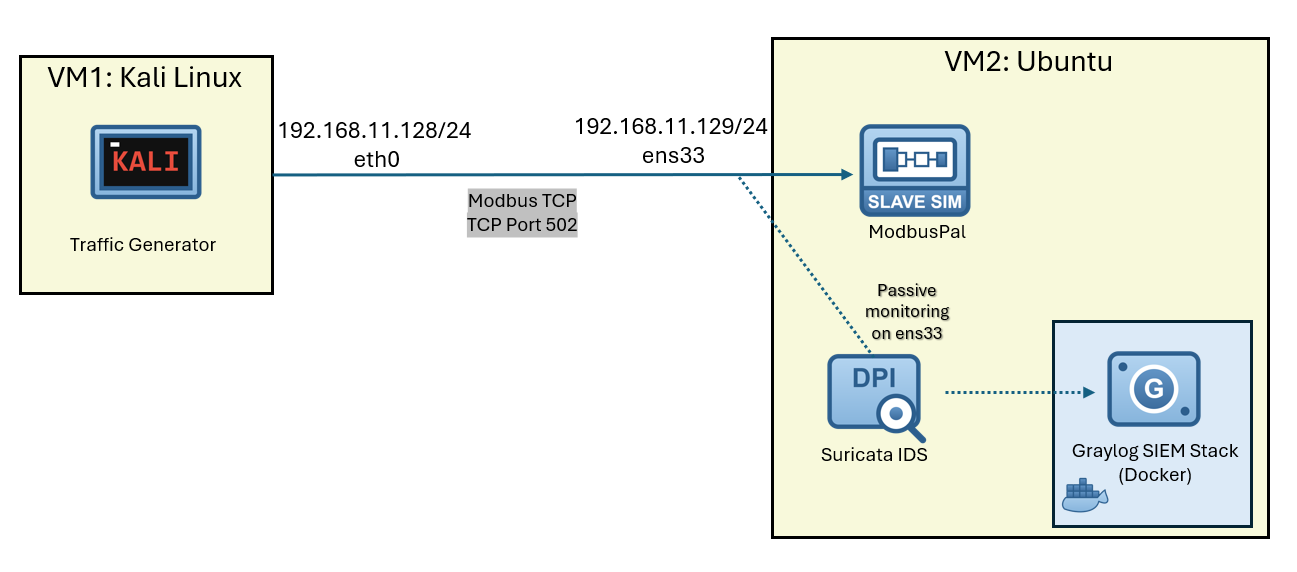
\includegraphics[width=\textwidth]{figure/Figure_5.2.png}
    \caption{Modbus TCP testbed with passive Suricata monitoring}
    \label{fig:Figure_5.2.jpg}
\end{figure}

\newpage
VM1 was assigned the IP address 192.168.11.128/24 on the eth0 interface and was responsible for generating Modbus TCP traffic. VM2 was assigned the IP address 192.168.11.129/24 on the ens33 interface and served as both the Modbus TCP target and the monitoring host. Since both virtual machines were located within the same subnet, Modbus TCP traffic could be transmitted directly from VM1 to VM2 without additional routing. The network configuration of the experimental testbed is summarized in Table \ref{tab:network_configuration}.

\begin{table}[htbp]
\caption{Network configuration of the experimental testbed}
\centering
\renewcommand{\arraystretch}{1.35}
\setlength{\tabcolsep}{6pt}
\resizebox{\linewidth}{!}{%
\begin{tabular}{|p{1cm}|p{3.4cm}|p{2.0cm}|p{3.8cm}|p{4.0cm}|p{5.0cm}|}
\hline
\textbf{Host} & \textbf{IP Address} & \textbf{Network Interface} & \textbf{Operating System} & \textbf{Role} & \textbf{Main Network Service} \\
\hline
VM1 & 192.168.11.128/24 & eth0 & Kali Linux 2025.04 & Attack host & Attack traffic generation \\
\hline
VM2 & 192.168.11.129/24 & ens33 & Ubuntu 22.04.5 LTS & PLC simulator / IDS / SIEM host & Modbus TCP service, IDS monitoring, SIEM collection \\
\hline
\end{tabular}%
}
\label{tab:network_configuration}
\end{table}

The ModbusPal PLC simulator was deployed on VM2 to provide the target Modbus TCP service over TCP port 502. All Modbus TCP requests generated from VM1 were sent to the simulated PLC service running on VM2. Suricata was also deployed on VM2 and configured to passively monitor the ens33 interface. In this configuration, Suricata operated as a network-based IDS and inspected Modbus TCP packets arriving at VM2 without acting as an inline gateway or forwarding device. Therefore, Suricata did not relay packets to ModbusPal; instead, it passively sniffed the traffic destined for the ModbusPal simulator.

\newpage
The generated Suricata events were written to the eve.json output file and subsequently collected by the Graylog SIEM stack for centralized event search, alert management, dashboard visualization, and analysis. Graylog was deployed on VM2 using Docker. This deployment allowed Modbus TCP traffic generation, IDS inspection, log collection, and SIEM-based event analysis to be evaluated within the same controlled virtual environment.

Before conducting the attack validation experiments, baseline Modbus TCP traffic was generated to verify the normal operation of the simulated PLC service and to establish a benign reference point for later comparison with malicious traffic. The purpose of the baseline validation was to confirm that normal Modbus TCP communication would not trigger the proposed Suricata detection rules.

To avoid ambiguity between legitimate write operations and unauthorized modification scenarios, the finalized baseline traffic was limited to normal Modbus TCP read operations. During preliminary compatibility testing, four common Modbus read function codes were considered: Read Coils 0x01, Read Discrete Inputs 0x02, Read Holding Registers 0x03, and Read Input Registers 0x04. However, under the current ModbusPal configuration, Read Input Registers 0x04 returned a Modbus exception response. Since Modbus exception responses are used as part of the proposed Scenario B detection logic, including 0x04 in the benign baseline would introduce abnormal protocol-level responses into the reference traffic. Therefore, function code 0x04 was excluded from the finalized benign baseline traffic. This exclusion was caused by the current ModbusPal configuration and does not indicate that FC04 is inherently abnormal in the Modbus protocol.

\newpage

As shown in Figure~\ref{fig:Figure_5.3.jpg}, the baseline script generated three rounds of Modbus TCP read requests from VM1 to VM2. In each round, Read Coils 0x01, Read Discrete Inputs 0x02, and Read Holding Registers 0x03 received normal responses from the ModbusPal simulator. This confirmed that the selected read function codes were supported by the simulator and were suitable for use as benign baseline traffic.

\begin{figure}[htbp]
    \centering
    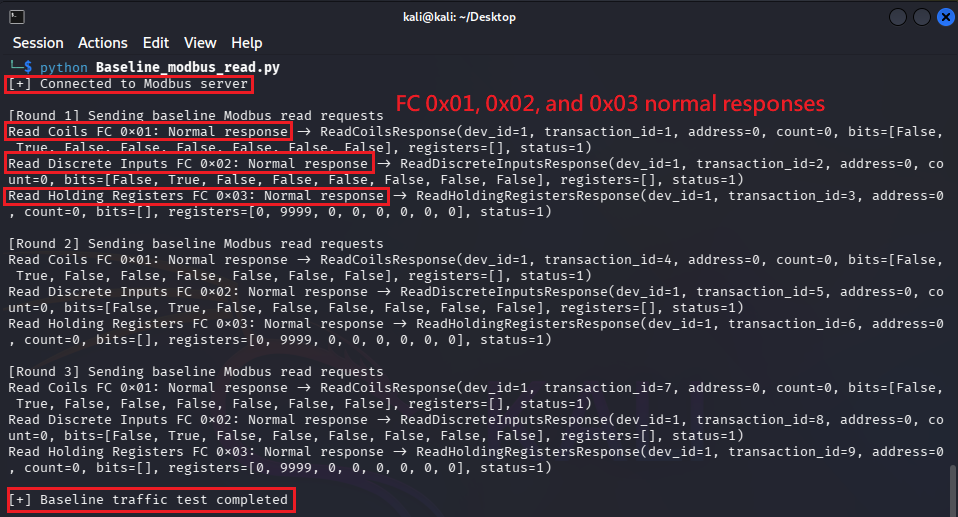
\includegraphics[width=\textwidth]{figure/Figure_5.3.png}
    \caption{Baseline Modbus TCP read requests showing normal responses for function codes 0x01, 0x02, and 0x03}
    \label{fig:Figure_5.3.jpg}
\end{figure}

\newpage

To further verify the baseline traffic at the packet level, tcpdump was executed on VM2 to capture traffic on the ens33 interface over TCP port 502. As shown in Figure~\ref{fig:Figure_5.4.jpg}, the captured packets show Modbus TCP communication between VM1 192.168.11.128 and VM2 192.168.11.129. The request payloads include the function codes 0x01, 0x02, and 0x03, confirming that the baseline read operations were transmitted over the network as expected.

\begin{figure}[htbp]
    \centering
    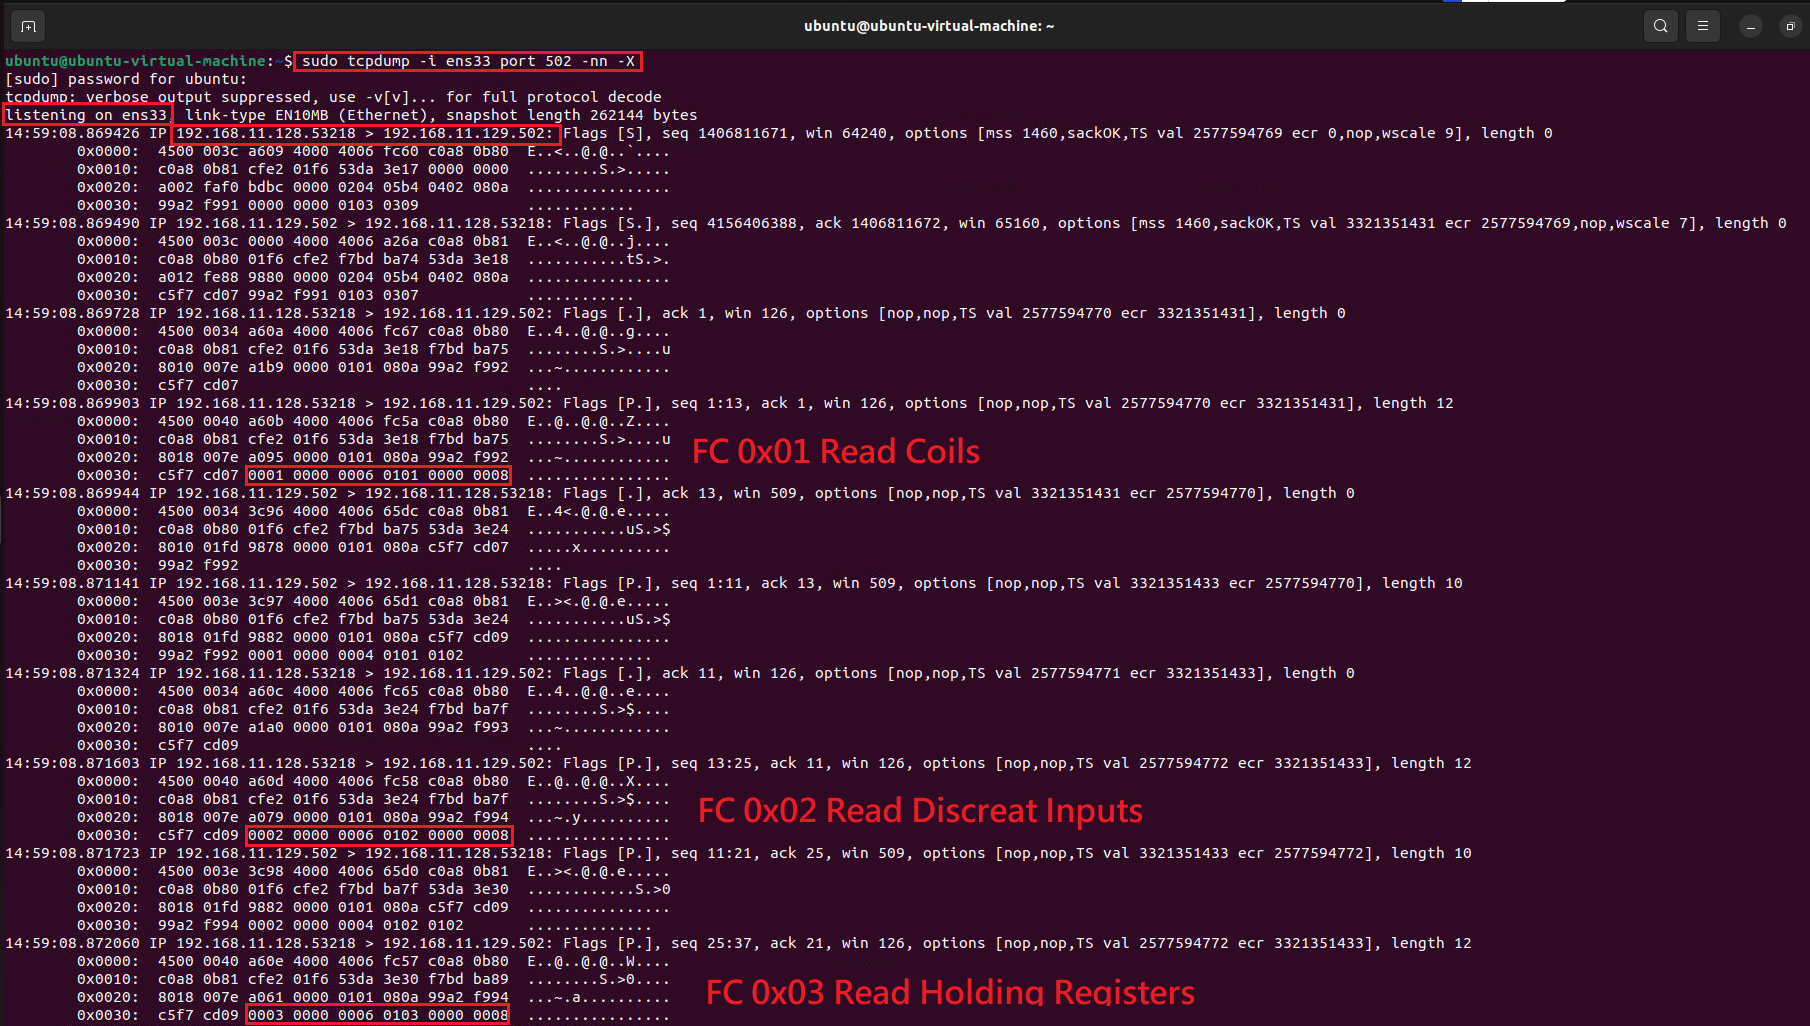
\includegraphics[width=\textwidth]{figure/Figure_5.4.png}
    \caption{tcpdump capture showing baseline Modbus TCP requests over TCP port 502}
    \label{fig:Figure_5.4.jpg}
\end{figure}
\newpage

After confirming the packet-level transmission of the baseline traffic, Suricata was monitored to verify whether any proposed detection rules were triggered during the same observation window. As shown in Figure~\ref{fig:Figure_5.5.jpg}, no alerts were generated in the Suricata fast.log output during the baseline validation. This result indicates that the finalized baseline traffic did not match the proposed detection rules and can therefore serve as a benign reference for subsequent attack scenario evaluation.

\begin{figure}[htbp]
    \centering
    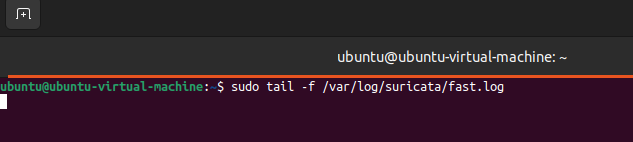
\includegraphics[width=\textwidth]{figure/Figure_5.5.png}
    \caption{Suricata fast.log output showing no alerts during baseline validation}
    \label{fig:Figure_5.5.jpg}
\end{figure}

The baseline validation results are summarized in Table \ref{tab:baseline_traffic_validation}. Overall, the finalized baseline traffic did not trigger the proposed Suricata detection rules. This result establishes a benign reference point for the subsequent attack scenario evaluation. It also confirms that alerts observed in later experiments can be attributed to abnormal Modbus behavior rather than normal baseline communication.

\begin{table}[htbp]
\caption{Baseline traffic validation result}
\centering
\renewcommand{\arraystretch}{1.35}
\setlength{\tabcolsep}{6pt}
\resizebox{\linewidth}{!}{%
\begin{tabular}{|p{4.2cm}|p{2cm}|p{3.cm}|p{3.6cm}|p{3.6cm}|}
\hline
\textbf{Traffic Type} & \textbf{Function Code} & \textbf{Number \newline of Rounds} & \textbf{Simulator \newline Response} & \textbf{Proposed \newline Suricata Alert} \\
\hline
Read Coils & 0x01 & 3 & Normal response & 0 \\
\hline
Read Discrete Inputs & 0x02 & 3 & Normal response & 0 \\
\hline
Read Holding Registers & 0x03 & 3 & Normal response & 0 \\
\hline
\end{tabular}%
}
\label{tab:baseline_traffic_validation}
\end{table}

Note. FC04 was excluded from the finalized baseline due to a ModbusPal configuration limitation that returned exception responses, not because FC04 is inherently abnormal.

\newpage

\section{Scenario-based Experimental Evaluation}
This section validates the eight scenario-based detection rules defined in Chapter 4 within a virtualized Modbus TCP test environment. The purpose of the experiment is to confirm whether Suricata can correctly detect anomalous features in Modbus TCP packets and whether Graylog can aggregate low-level Suricata alerts into high-level events with OT security semantics.

The experimental scenarios cover the Test, Deliver, Install / Modify, and Execute ICS Attack stages of ICS Cyber Kill Chain Stage 2. They are mapped to FR 2, FR 3, FR 5, and FR 7 of ISA/IEC 62443-3-3, as well as MITRE ATT\&CK for ICS techniques including Remote System Discovery, Modify Parameter, Manipulation of Control, Device Restart/Shutdown, and Denial of Service. Table \ref{tab:rule_suricata_mapping} summarizes the experimental scenarios, trigger conditions, Suricata SIDs, Graylog priorities, and expected results.

\begin{table}[htbp]
\caption{Mapping of Detection Rules to Suricata SIDs and Graylog Alert Priorities}
\centering
\footnotesize
\renewcommand{\arraystretch}{1.5}

\resizebox{\textwidth}{!}{%
\begin{tabular}{|>{\centering\arraybackslash}m{1.1cm}|>{\bfseries\centering\arraybackslash}m{0.9cm}|>{\centering\arraybackslash}m{2.4cm}|>{\centering\arraybackslash}m{3.4cm}|>{\centering\arraybackslash}m{1.7cm}|>{\centering\arraybackslash}m{1.5cm}|>{\centering\arraybackslash}m{2.8cm}|}
\hline
\textbf{Section} & \textbf{Rule ID} & \textbf{Scenario} & \textbf{Trigger Condition} & \textbf{Suricata SID} & \textbf{Graylog Priority} & \textbf{Expected Result} \\ \hline

5.2.1 & A & Reconnaissance Scanning & FC17 or FC43 probing request & 1000101, 1000102 & Normal & Reconnaissance alert is triggered. \\ \hline

5.2.2 & B1 & Request-side Modbus Protocol Probing & Unsupported Function Code or MBAP Protocol ID not equal to \texttt{0x0000} & 1000201, 1000202 & Normal & Protocol probing alert is triggered. \\ \hline

5.2.3 & B2 & Response-side Modbus Exception & Exception Code \texttt{0x01} to \texttt{0x0B} returned by server & 1000203--1000212 & Normal & Exception response alert is triggered. \\ \hline

5.2.4 & C1 & Unauthorized Modification & FC05, FC06, FC15, or FC16 write operation & 1000301--1000304 & High & Unauthorized modification alert is triggered. \\ \hline

5.2.5 & C2 & Advanced Register Manipulation & FC22 or FC23 advanced register operation & 1000305, 1000306 & High & Register manipulation alert is triggered. \\ \hline

5.2.6 & D & Critical Diagnostic Command Injection & FC08 sub-function \texttt{0x0001}, \texttt{0x0004}, or \texttt{0x000A} & 1000404--1000406 & High & Critical diagnostic command alert is triggered. \\ \hline

5.2.7 & E1 & High-rate SYN Activity & TCP/502 SYN packets exceed threshold & 1000501 & High & Connection-layer DoS alert is triggered. \\ \hline

5.2.8 & E2 & High-rate Payload Activity & TCP/502 payload-bearing packets exceed threshold & 1000502 & High & Application-layer DoS alert is triggered. \\ \hline

\end{tabular}%
}
\label{tab:rule_suricata_mapping}
\end{table}


\newpage

\subsection{Scenario A - Reconnaissance Scanning}
In this scenario, the Nmap Modbus discovery script was first executed against the target device to generate FC17 Report Server ID and FC43 Read Device Identification requests, simulating an attacker collecting device identity, service information, and supported capabilities before an attack. After the attack was executed, Suricata successfully detected the FC17 and FC43 requests, and Graylog aggregated the related events into a Reconnaissance Scanning alert. Figure~\ref{fig:Figure_5.6_A-1.png} shows the attack execution, and Figure~\ref{fig:Figure_5.7_A-2.png} shows the corresponding detection result in Graylog.

This scenario corresponds to the Test stage of ICS Cyber Kill Chain Stage 2, FR 5 Restricted Data Flow in ISA/IEC 62443-3-3, and T0846 Remote System Discovery in MITRE ATT\&CK for ICS.

\begin{figure}[H]
    \centering
    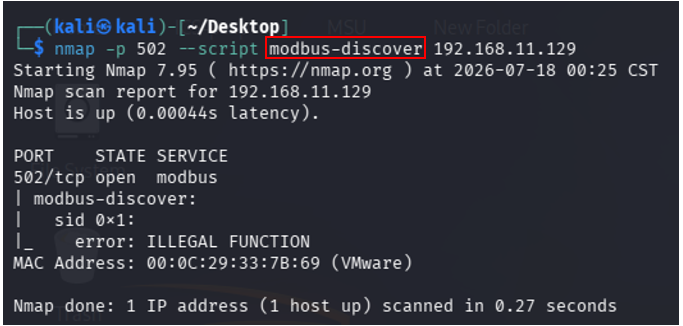
\includegraphics[width=0.9\textwidth]{figure/Figure_5.6_A-1.png}
    \caption{Attack execution of Scenario A using Nmap Modbus discovery}
    \label{fig:Figure_5.6_A-1.png}
\end{figure}

\begin{figure}[H]
    \centering
    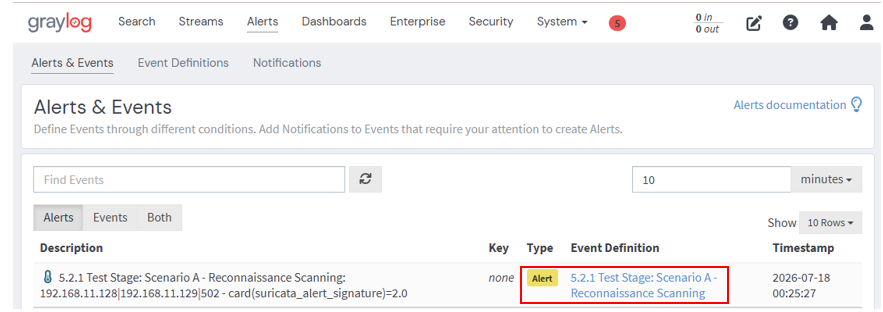
\includegraphics[width=0.9\textwidth]{figure/Figure_5.7_A-2.png}
    \caption{Detection result of Scenario A reconnaissance scanning in Graylog}
    \label{fig:Figure_5.7_A-2.png}
\end{figure}

\newpage

\subsection{Scenario B1 - Request-side Modbus Protocol Probing}
This scenario simulated Modbus protocol probing or fuzzing through abnormal Modbus requests. The attack packets included unsupported Function Codes and malformed requests whose MBAP Protocol Identifier was not 0x0000, testing how the target device handled non-standard requests. After the attack was executed, Suricata detected the abnormal requests based on the MBAP header and PDU Function Code and triggered Scenario B1 alerts. Graylog then aggregated the related events into Request-side Modbus Protocol Probing. Figure~\ref{fig:Figure_5.8_B1-1.png} shows the attack execution, and Figure~\ref{fig:Figure_5.9_B1-2.png} shows the corresponding detection result.

This scenario corresponds to the Delivery stage of ICS Cyber Kill Chain Stage 2, FR 3 System Integrity in ISA/IEC 62443-3-3, and T0846 Remote System Discovery in MITRE ATT\&CK for ICS.

\begin{figure}[H]
    \centering
    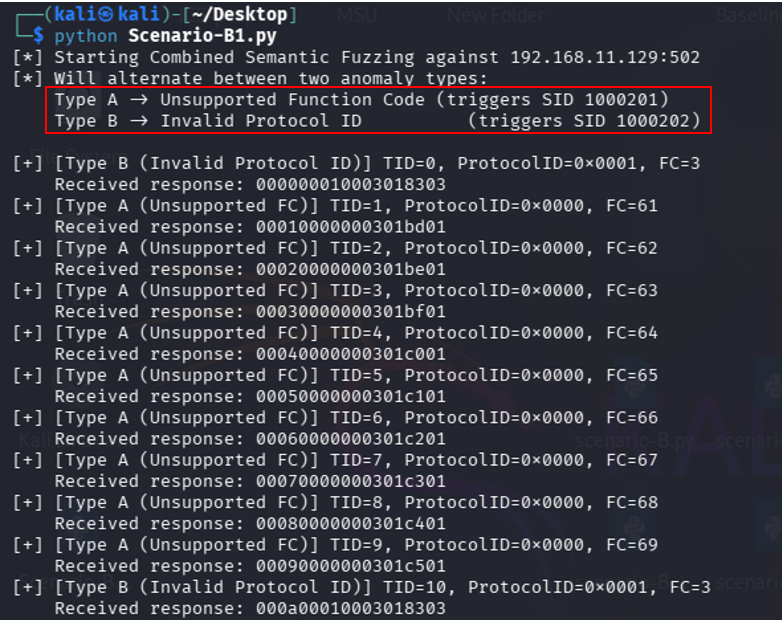
\includegraphics[width=0.9\textwidth]{figure/Figure_5.8_B1-1.png}
    \caption{Attack execution of Scenario B1 using malformed Modbus requests}
    \label{fig:Figure_5.8_B1-1.png}
\end{figure}

\begin{figure}[H]
    \centering
    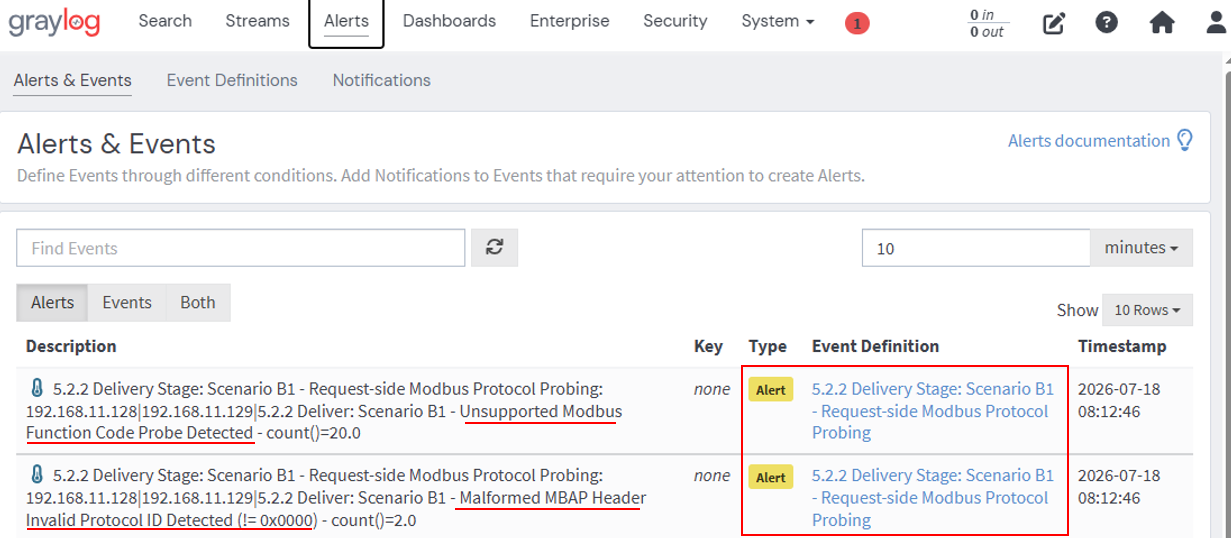
\includegraphics[width=0.95\textwidth]{figure/Figure_5.9_B2-2.png}
    \caption{Detection result of Scenario B1 request-side protocol probing in Graylog}
    \label{fig:Figure_5.9_B1-2.png}
\end{figure}

\newpage

\subsection{Scenario B2 - Response-side Modbus Exception Detection}
In this scenario, the attacker sent unsupported Function Codes, illegal addresses, or invalid data values to cause the Modbus server to return corresponding Exception Responses, simulating an attacker observing error responses through abnormal requests. After the attack was executed, Suricata successfully detected multiple Modbus Exception Codes, and Graylog aggregated the related alerts into the Response-side Modbus Exception Detection scenario. Figure~\ref{fig:Figure_5.10_B2-1.png} shows the attack execution, and Figure~\ref{fig:Figure_5.11_B2-2.png} shows the detection result in Graylog.

This scenario corresponds to the Delivery stage of ICS Cyber Kill Chain Stage 2, FR 3 System Integrity in ISA/IEC 62443-3-3, and T0846 Remote System Discovery in MITRE ATT\&CK for ICS.

\begin{figure}[H]
    \centering
    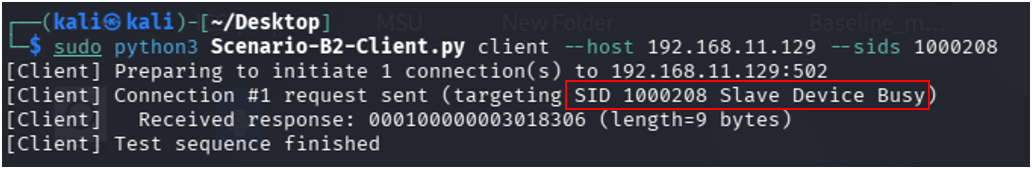
\includegraphics[width=0.9\textwidth]{figure/Figure_5.10_B2-1.png}
    \caption{ Attack execution of Scenario B2 triggering Modbus exception responses}
    \label{fig:Figure_5.10_B2-1.png}
\end{figure}

\begin{figure}[H]
    \centering
    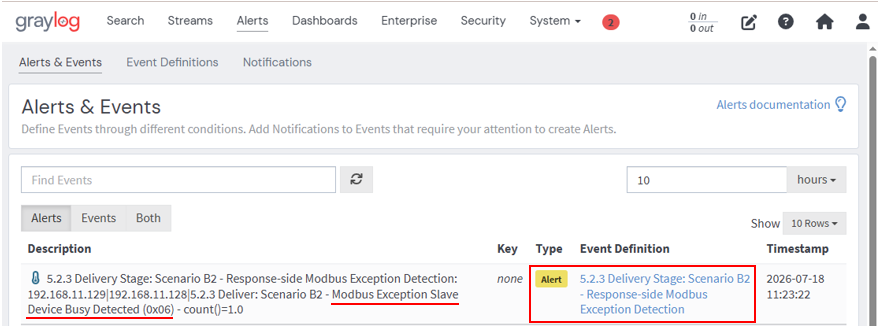
\includegraphics[width=0.9\textwidth]{figure/Figure_5.11_B2-2.png}
    \caption{Detection result of Scenario B2 Modbus exception response in Graylog}
    \label{fig:Figure_5.11_B2-2.png}
\end{figure}

\subsection{Scenario C1 - Unauthorized Modification}
In this scenario, Modbus write commands were sent from an unauthorized source to the target device, including FC05 Write Single Coil, FC06 Write Single Register, FC15 Write Multiple Coils, and FC16 Write Multiple Registers. This simulated an attacker attempting to modify coil states or holding register values. After the attack was executed, Suricata successfully detected the write-related Function Codes, and Graylog further identified the source as unauthorized based on source IP and whitelist conditions, generating a high-priority Unauthorized Modification alert. Figure~\ref{fig:Figure_5.12_C1-1.png} shows the attack execution, and Figure~\ref{fig:Figure_5.13_C1-2.png} shows the detection result in Graylog.

This scenario corresponds to the Install/Modify stage of ICS Cyber Kill Chain Stage 2, FR 2 Use Control in ISA/IEC 62443-3-3, and T0836 Modify Parameter in MITRE ATT\&CK for ICS.
\begin{figure}[H]
    \centering
    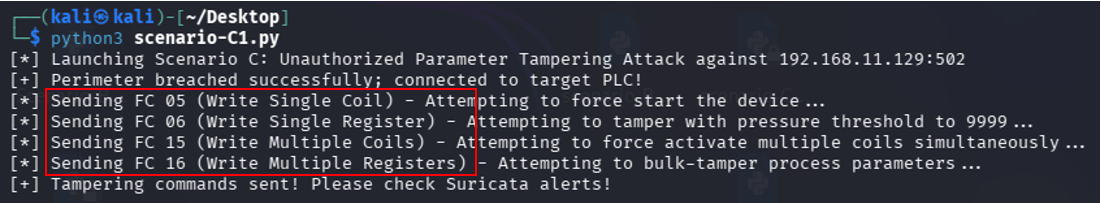
\includegraphics[width=0.9\textwidth]{figure/Figure_5.12_C1-1.png}
    \caption{Attack execution of Scenario C1 unauthorized Modbus write operation}
    \label{fig:Figure_5.12_C1-1.png}
\end{figure}
\begin{figure}[H]
    \centering
    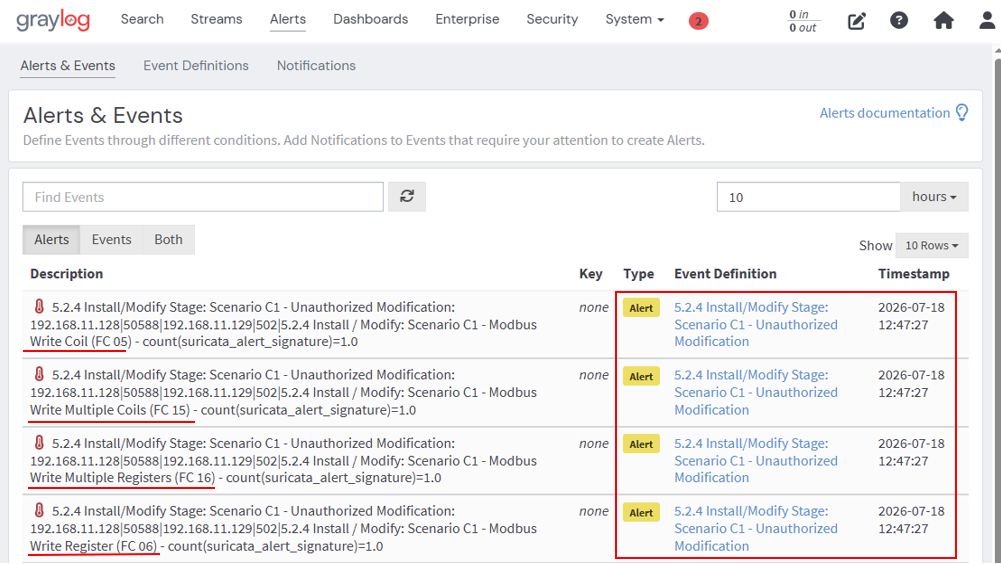
\includegraphics[width=0.85\textwidth]{figure/Figure_5.13_C1-2.png}
    \caption{Detection result of Scenario C1 unauthorized modification in Graylog}
    \label{fig:Figure_5.13_C1-2.png}
\end{figure}
\newpage

\subsection{Scenario C2 - Advanced Register Manipulation}
In this scenario, FC22 Mask Write Register and FC23 Read/Write Multiple Registers were sent to the target device to simulate advanced manipulation, such as bit-level modification or combined reading and writing of multiple registers within a single transaction. After the attack was executed, Suricata correctly identified FC22 and FC23 through the PDU Function Code, and Graylog classified the related events as Advanced Register Manipulation. Figure~\ref{fig:Figure_5.14_C2-1.png} shows the attack execution, and Figure~\ref{fig:Figure_5.15_C2-2.png} shows the corresponding detection result.

This scenario corresponds to the Install/Modify stage of ICS Cyber Kill Chain Stage 2, FR 3 System Integrity in ISA/IEC 62443-3-3, and T0831 Manipulation of Control in MITRE ATT\&CK for ICS.

\begin{figure}[H]
    \centering
    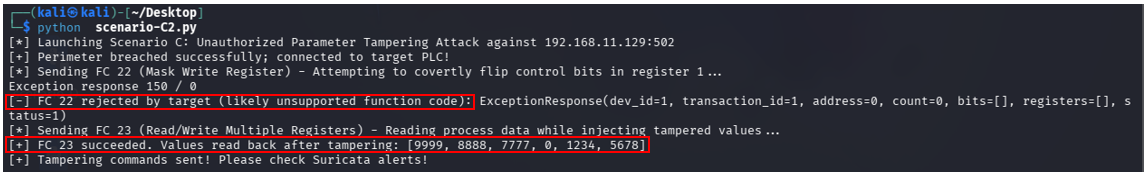
\includegraphics[width=1.0\textwidth]{figure/Figure_5.14_C2-1.png}
    \caption{Attack execution of Scenario C2 advanced register manipulation}
    \label{fig:Figure_5.14_C2-1.png}
\end{figure}

\begin{figure}[H]
    \centering
    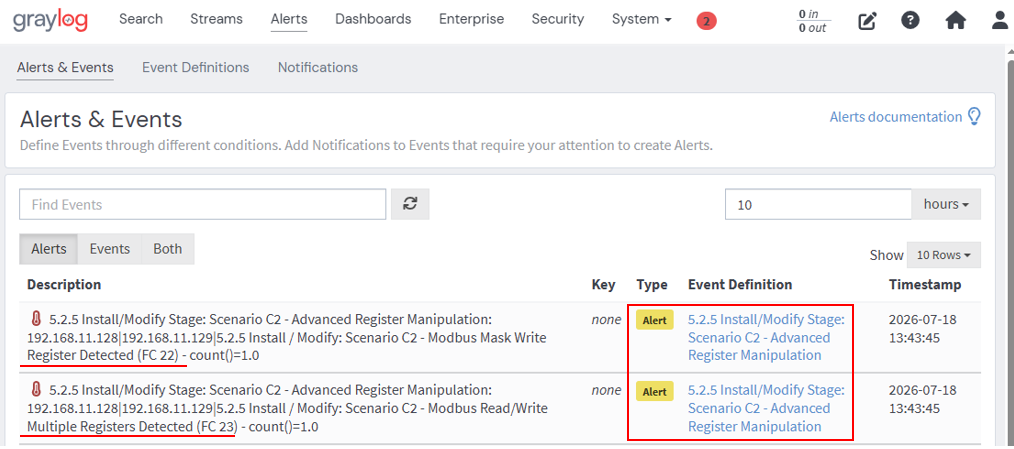
\includegraphics[width=1.0\textwidth]{figure/Figure_5.15_C2-2.png}
    \caption{Detection result of Scenario C2 advanced register manipulation in Graylog}
    \label{fig:Figure_5.15_C2-2.png}
\end{figure}

\subsection{Scenario D - Critical Diagnostic Command Injection}
In this scenario, high-risk sub-functions within Modbus FC08 Diagnostic commands were sent to the target device, including 0x0001 Restart Communications Option, 0x0004 Force Listen Only Mode, and 0x000A Clear Counters and Diagnostic Register. These commands simulated communication reinitialization, listen-only mode, and diagnostic information clearing. After the attack was executed, Suricata not only identified FC08 but also successfully parsed the sub-function field in the PDU and generated alerts when high-risk conditions were matched. Graylog aggregated the events into a high-priority Critical Diagnostic Command Injection alert. Figure~\ref{fig:Figure_5.16_D-1.png} shows the attack execution, and Figure~\ref{fig:Figure_5.17_D-2.png} shows the detection result in Graylog.

This scenario corresponds to the Execute ICS Attack stage of ICS Cyber Kill Chain Stage 2, FR 3 System Integrity in ISA/IEC 62443-3-3, and T0816 Device Restart/Shutdown in MITRE ATT\&CK for ICS.

\begin{figure}[H]
    \centering
    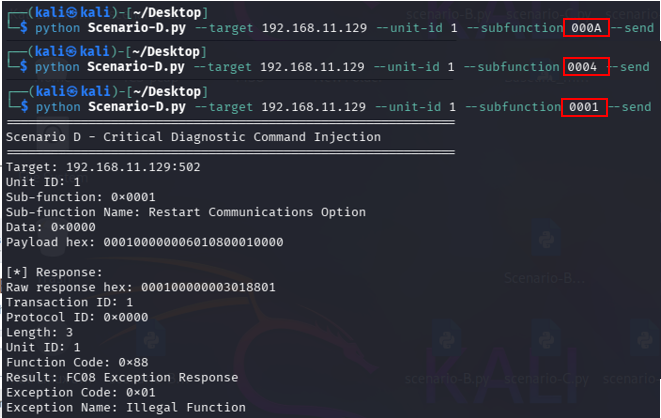
\includegraphics[width=1.0\textwidth]{figure/Figure_5.16_D-1.png}
    \caption{Attack execution of Scenario D critical diagnostic command injection}
    \label{fig:Figure_5.16_D-1.png}
\end{figure}

\begin{figure}[H]
    \centering
    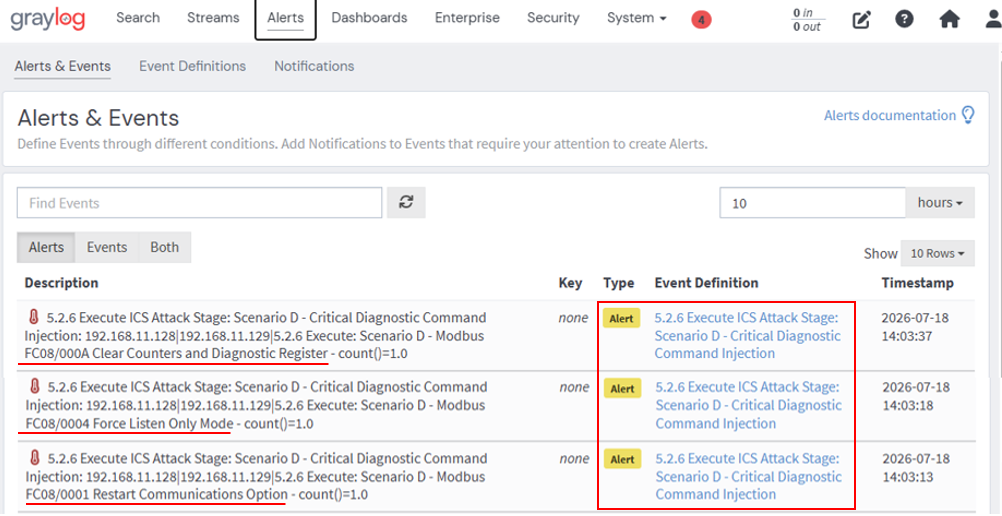
\includegraphics[width=1.0\textwidth]{figure/Figure_5.17_D-2.png}
    \caption{Detection result of Scenario D critical diagnostic command injection in Graylog}
    \label{fig:Figure_5.17_D-2.png}
\end{figure}
\newpage


\subsection{Scenario E1 - Modbus TCP/502 High-rate SYN Activity}
In this scenario, a large number of TCP SYN packets were sent to Modbus TCP port 502 to simulate a connection-layer DoS attack that consumes connection-handling resources of the target device. After the attack was executed, Suricata counted SYN packets within a short time window using a threshold condition and triggered a High-rate SYN Activity alert when the same source exceeded the configured threshold. Graylog then classified the event as DoS behavior in the Execute ICS Attack stage. Figure~\ref{fig:Figure_5.18_E1-1.png} shows the attack execution, and Figure Figure~\ref{fig:Figure_5.19_E1-2.png} shows the detection result in Graylog.

This scenario corresponds to the Execute ICS Attack stage of ICS Cyber Kill Chain Stage 2, FR 7 Resource Availability in ISA/IEC 62443-3-3, and T0814 Denial of Service in MITRE ATT\&CK for ICS.

\begin{figure}[H]
    \centering
    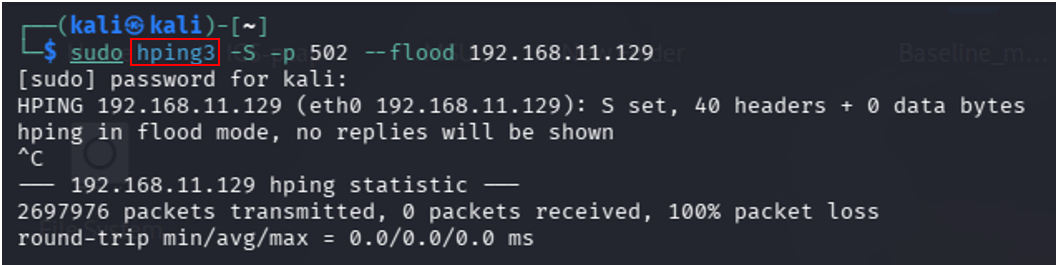
\includegraphics[width=1.0\textwidth]{figure/Figure_5.18_E1-1.png}
    \caption{Attack execution of Scenario E1 high-rate SYN activity against Modbus TCP/502}
    \label{fig:Figure_5.18_E1-1.png}
\end{figure}

\begin{figure}[H]
    \centering
    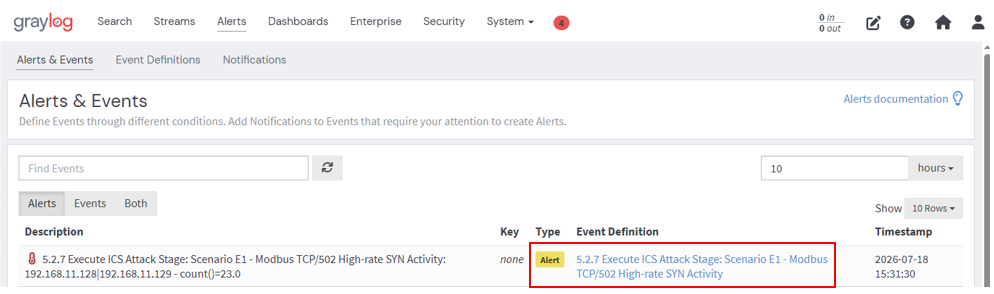
\includegraphics[width=1.0\textwidth]{figure/Figure_5.19_E1-2.png}
    \caption{Detection result of Scenario E1 high-rate SYN activity in Graylog}
    \label{fig:Figure_5.19_E1-2.png}
\end{figure}

\subsection{Scenario E2 - Modbus TCP/502 High-rate Payload Activity}
In this scenario, a large number of TCP packets containing payloads were sent to Modbus TCP port 502 to simulate a service stress attack that forces the Modbus server to continuously parse and process application-layer requests. After the attack was executed, Suricata confirmed payload-bearing packets using the dsize condition and combined it with a threshold to count packets within a defined time window. When the traffic exceeded the threshold, the system triggered a High-rate Payload Activity alert. This scenario complements Scenario E1 by covering application-layer DoS behavior after connections have been established. Figure~\ref{fig:Figure_5.20_E2-1.png} shows the attack execution, and Figure~\ref{fig:Figure_5.21_E2-2.png} shows the detection result in Graylog.

This scenario corresponds to the Execute ICS Attack stage of ICS Cyber Kill Chain Stage 2, FR 7 Resource Availability in ISA/IEC 62443-3-3, and T0814 Denial of Service in MITRE ATT\&CK for ICS.

\begin{figure}[H]
    \centering
    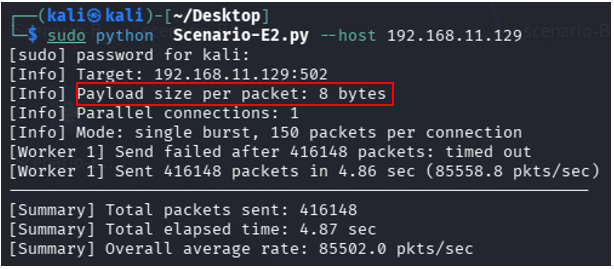
\includegraphics[width=1.0\textwidth]{figure/Figure_5.20_E2-1.png}
    \caption{Attack execution of Scenario E1 high-rate SYN activity against Modbus TCP/502}
    \label{fig:Figure_5.20_E2-1.png}
\end{figure}

\begin{figure}[H]
    \centering
    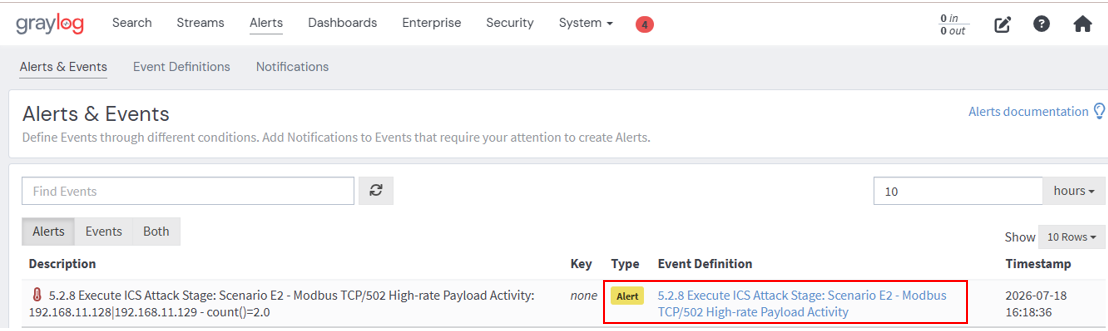
\includegraphics[width=1.0\textwidth]{figure/Figure_5.21_E2-2.png}
    \caption{Detection result of Scenario E1 high-rate SYN activity in Graylog}
    \label{fig:Figure_5.21_E2-2.png}
\end{figure}

\newpage

\subsection{Detection Results Summary}
This section summarizes the triggering results of the scenario-based detection rules in the experimental environment. Suricata generated alerts based on the MBAP header, Function Code, Exception Code, diagnostic sub-function, and TCP connection features in Modbus TCP packets. Graylog then aggregated these alerts into scenario-based events using signatures, time windows, source addresses, and priority conditions.

As shown in Table \ref{tab:security_meaning}, the scenario-based rules were successfully triggered. Reconnaissance scanning, protocol probing, and abnormal responses mainly represent early-stage attack activities and were assigned Normal priority. Unauthorized modification, advanced register manipulation, diagnostic command injection, and service availability impacts involve device state, integrity, or availability and were assigned High priority. The results show that the proposed framework can transform Modbus packet-level anomalies into more understandable and actionable scenario-based alerts.

The detection conditions are complementary, supporting monitoring of probing behavior, control operations, and resource availability in OT environments.

Overall, the results confirm that the proposed framework can detect Modbus TCP attack behaviors across different stages of the ICS Cyber Kill Chain. Suricata provided protocol-aware detection, while Graylog supported centralized alert presentation and severity classification. The next section further discusses how Graylog correlates these alerts and provides SIEM-based operational visibility.

\begin{table}[htbp]
\caption{Security Meaning and Validation Summary of Proposed Detection Rules}
\centering
\footnotesize
\renewcommand{\arraystretch}{1.5}

\resizebox{\textwidth}{!}{%
\begin{tabular}{|>{\bfseries\centering\arraybackslash}m{0.7cm}|>{\centering\arraybackslash}m{2.6cm}|>{\centering\arraybackslash}m{2.2cm}|>{\centering\arraybackslash}m{2.4cm}|>{\centering\arraybackslash}m{2.6cm}|>{\centering\arraybackslash}m{1.3cm}|>{\centering\arraybackslash}m{1.3cm}|}
\hline
\textbf{Rule ID} & \textbf{Scenario} & \textbf{ICS Cyber Kill Chain} & \textbf{ISA/IEC 62443-3-3 FR} & \textbf{MITRE ATT\&CK for ICS} & \textbf{Priority} & \textbf{Lab Result} \\ \hline

A & Reconnaissance Scanning & Stage 2: \newline Test & FR 5 - Restrict Data Flow & T0846 - Remote System Discovery & Normal & Triggered \\ \hline

B1 & Request-side Modbus Protocol Probing & Stage 2: Deliver & FR 3 - System Integrity & T0846 - Remote System Discovery & Normal & Triggered \\ \hline

B2 & Response-side Modbus Exception Detection & Stage 2: Deliver & FR 3 - System Integrity & T0846 - Remote System Discovery & Normal & Triggered \\ \hline

C1 & Unauthorized Modification & Stage 2: Install / Modify & FR 2 - Use Control & T0836 - Modify Parameter & High & Triggered \\ \hline

C2 & Advanced Register Manipulation & Stage 2: Install / Modify & FR 3 - System Integrity & T0831 - Manipulation of Control & High & Triggered \\ \hline

D & Critical Diagnostic Command Injection & Stage 2: Execute ICS Attack & FR 3 - System Integrity & T0816 - Device Restart/Shutdown & High & Triggered \\ \hline

E1 & High-rate SYN Activity & Stage 2: Execute ICS Attack & FR 7 - Resource Availability & T0814 - Denial of Service & High & Triggered \\ \hline

E2 & High-rate Payload Activity & Stage 2: Execute ICS Attack & FR 7 - Resource Availability & T0814 - Denial of Service & High & Triggered \\ \hline

\end{tabular}%
}
\label{tab:security_meaning}
\end{table}

\newpage

\section{SIEM Alert Correlation and Traceability Analysis}

In Section 5.2, the proposed Suricata rules were validated against five Modbus TCP attack scenarios. This section further analyzes how Graylog supports SIEM-based correlation, event traceability, dashboard visualization, and instant notification. In the proposed framework, Suricata performs packet-level detection, while Graylog correlates alerts into scenario-level security events with additional context such as source IP, destination IP, rule name, severity, attack type, and framework mapping.

\subsection{Graylog Correlation Rule Analysis}
This research establishes scenario-based correlation rules in Graylog, corresponding to the experimental scenarios in Sections 5.2.1 to 5.2.8. These rules do not merely duplicate individual packet alerts generated by Suricata. Instead, they aggregate Suricata signatures according to attack stage, detection objective, and OT security semantics, making the alert results more suitable for industrial control system operations and security monitoring.

To clarify how Suricata signatures are aggregated into scenario-based alerts, Table~\ref{tab:siem_correlation_logic} summarizes the SIEM correlation logic adopted in this study. The correlation logic covers multi-event reconnaissance, protocol anomaly detection, whitelist-based command validation, deep protocol field inspection, and rate-based traffic detection. These logic types provide the basis for transforming low-level packet alerts into higher-level attack scenarios within Graylog.
\begin{table}[H]
\caption{SIEM Detection Logic for Scenario-based Correlation Rules}
\centering
\small
\begin{tabularx}{\linewidth}{|l|>{\hsize=0.8\hsize}X|>{\hsize=1.4\hsize}X|>{\hsize=0.8\hsize}X|}
\hline
\textbf{No.} & \textbf{Detection Logic} & \textbf{Graylog Correlation Logic} & \textbf{Interpretation} \\
\hline
A & Device \newline identification \newline correlation 
& FC17 Report Server ID and FC43 Read Device Identification requests from the same source 
& Modbus device \newline fingerprinting \\
\hline
B & Protocol anomaly \newline aggregation 
& Unsupported FCs, invalid MBAP Protocol ID, malformed fields, or Modbus exception responses 
& Protocol probing \newline and fuzzing \\
\hline
C & Write-command \newline validation 
& FC05, FC06, FC15, FC16, FC22, and FC23 from \newline non-whitelisted or unexpected IPs 
& Unauthorized \newline modification \\
\hline
D & Diagnostic \newline sub-function \newline inspection 
& FC08 diagnostic sub-functions, such as Restart Communications and Force Listen Only Mode 
& Critical diagnostic \newline command injection \\
\hline
E & Rate-threshold \newline detection 
& High-rate TCP SYN packets or payload-bearing Modbus TCP requests targeting port 502 
& DoS flooding or \newline service stress \\
\hline
\end{tabularx}
\label{tab:siem_correlation_logic}
\end{table}






\newpage
To further summarize the overall distribution of the Graylog correlation rules, Table~\ref{tab:rule_category_summary} presents the number of rules, corresponding sections, and priority settings for each detection category. Based on the alert severity classification defined in Section 4.4.1, Scenario A, B1, and B2 are assigned Normal priority and are mainly used to identify reconnaissance, protocol probing, and abnormal responses. These events may not immediately cause process disruption, but they serve as important indicators of early-stage attack activity. Scenario C1, C2, D, E1, and E2 are assigned High priority because they involve control parameter modification, advanced register operations, diagnostic command abuse, or impacts on service availability, which pose higher operational risks to OT environments.
\begin{table}[htbp]
\caption{Summary of Detection Rule Categories and Corresponding Priorities}
\centering
\footnotesize
\renewcommand{\arraystretch}{1.5}

\resizebox{\textwidth}{!}{%
\begin{tabular}{|>{\centering\arraybackslash}m{5.0cm}|>{\centering\arraybackslash}m{2.2cm}|>{\centering\arraybackslash}m{2.6cm}|>{\centering\arraybackslash}m{1.8cm}|}
\hline
\textbf{Category} & \textbf{Number of Rules} & \textbf{Corresponding Sections} & \textbf{Priority} \\ \hline

Reconnaissance and Discovery & 1 & 5.2.1 & Normal \\ \hline

Protocol Probing and Exception Detection & 2 & 5.2.2--5.2.3 & Normal \\ \hline

Unauthorized Modification and Register Manipulation & 2 & 5.2.4--5.2.5 & High \\ \hline

Diagnostic Command Injection & 1 & 5.2.6 & High \\ \hline

Denial-of-Service Detection & 2 & 5.2.7--5.2.8 & High \\ \hline\hline

\textbf{Total} & \textbf{8} & \textbf{5.2.1--5.2.8} & \textbf{Normal--High} \\ \hline

\end{tabular}%
}
\label{tab:rule_category_summary}
\end{table}

Overall, the Graylog correlation rules transform low-level Suricata events into high-level alerts mapped to the ICS Cyber Kill Chain, ISA/IEC 62443-3-3, and MITRE ATT\&CK for ICS. As shown in Table~\ref{tab:table5_11}, each rule is described with its scenario name, primary detection field, security framework mapping, priority, laboratory result, and security meaning.
\begin{table}[htbp]
\caption{Security Mapping and Meaning of Proposed Detection Rules}
\centering
\footnotesize
\renewcommand{\arraystretch}{1.45}

\resizebox{\textwidth}{!}{%
\begin{tabular}{|>{\bfseries\centering\arraybackslash}m{0.9cm}
                |>{\centering\arraybackslash}m{3.2cm}
                |>{\centering\arraybackslash}m{2.4cm}
                |>{\centering\arraybackslash}m{2.5cm}
                |>{\centering\arraybackslash}m{3.0cm}
                |>{\centering\arraybackslash}m{5.0cm}|}
\hline
\textbf{Rule ID} & 
\textbf{Scenario} & 
\textbf{ICS Cyber Kill Chain Stage} & 
\textbf{ISA/IEC 62443-3-3} & 
\textbf{MITRE ATT\&CK for ICS} & 
\textbf{Security Meaning} \\ 
\hline

A & Reconnaissance Scanning 
& Test 
& FR 5 -- Restrict Data Flow 
& T0846 -- Remote System Discovery 
& Detects device identification and remote system discovery behavior. \\ 
\hline

B1 & Request-side Modbus Protocol Probing 
& Deliver 
& FR 3 -- System Integrity 
& T0846 -- Remote System Discovery 
& Detects malformed requests and protocol probing. \\ 
\hline

B2 & Response-side Modbus Exception Detection 
& Deliver 
& FR 3 -- System Integrity 
& T0846 -- Remote System Discovery 
& Detects device exception responses caused by abnormal requests. \\ 
\hline

C1 & Unauthorized Modification 
& Install / Modify 
& FR 2 -- Use Control 
& T0836 -- Modify Parameter 
& Detects unauthorized coil or register write operations. \\ 
\hline

C2 & Advanced Register Manipulation 
& Install / Modify 
& FR 3 -- System Integrity 
& T0831 -- Manipulation of Control 
& Detects advanced register manipulation and control parameter modification. \\ 
\hline

D & Critical Diagnostic Command Injection 
& Execute ICS Attack 
& FR 3 -- System Integrity 
& T0816 -- Device Restart/Shutdown 
& Detects high-risk diagnostic commands and device communication disruption. \\ 
\hline

E1 & High-rate SYN Activity 
& Execute ICS Attack 
& FR 7 -- Resource Availability 
& T0814 -- Denial of Service 
& Detects connection-layer DoS attacks. \\ 
\hline

E2 & High-rate Payload Activity 
& Execute ICS Attack 
& FR 7 -- Resource Availability 
& T0814 -- Denial of Service 
& Detects application-layer Modbus service stress attacks. \\ 
\hline

\end{tabular}%
}
\label{tab:table5_11}
\end{table}

\newpage

\subsection{Severity, Confidence, and Framework Mapping}
This study distinguishes between alert severity and alert confidence. As shown in Table~\ref{tab:severity_confidence}, severity represents the potential operational impact of an event, while confidence represents the strength of supporting evidence behind the alert. Therefore, these two concepts were treated separately in the alert evaluation process.

Severity was determined based on the attack behavior, ICS Cyber Kill Chain stage, and ISA/IEC 62443-3-3 Foundational Requirement. Scenarios A and B were classified as Normal severity because they belong to early-stage reconnaissance and delivery behaviors. In contrast, Scenarios C, D, and E were classified as High severity because they may affect system integrity, control behavior, or resource availability.

Confidence was improved through SIEM correlation. For example, repeated events from the same source, temporal correlation within a defined time window, whitelist violations, protocol field matching, and threshold-based traffic patterns all provide additional evidence for alert interpretation. This design helps reduce isolated and low-context alerts by associating them with supporting event patterns.

MITRE ATT\&CK for ICS was used as a supplementary TTP mapping reference rather than as the primary detection logic. This mapping helps analysts interpret detected Modbus TCP events in terms of attack techniques and behavior context.

\begin{table}[H]
\caption{Difference between Alert Severity and Alert Confidence}
\centering
\begin{tabular}{|l|l|p{6cm}|}
\hline
\textbf{Item} & \textbf{Meaning} & \textbf{Determination Basis} \\
\hline
Severity & Potential operational impact & Kill Chain stage, attack type, and ISA/IEC 62443-3-3 FR \\
\hline
Confidence & Strength of supporting evidence & Time window, repeated events, whitelist violation, protocol field matching, and threshold patterns \\
\hline
\end{tabular}
\label{tab:severity_confidence}
\end{table}

\subsection{Graylog Visualization and Instant Notification}

Graylog provided dashboard visualization for monitoring Modbus TCP security events. As shown in Figure~\ref{fig:Figure_5.22.png}, the dashboard presents key information such as event time, source IP, destination IP, rule name, attack type, severity, and scenario mapping. These fields allow operators to quickly identify abnormal behaviors and trace the related communication context.

The dashboard also improves operational visibility by allowing alerts to be filtered according to scenario, severity, source IP, destination IP, or rule name. Therefore, operators can distinguish whether an event is related to reconnaissance, protocol fuzzing, unauthorized modification, command injection, or denial-of-service activity.

\begin{figure}[H]
    \centering
    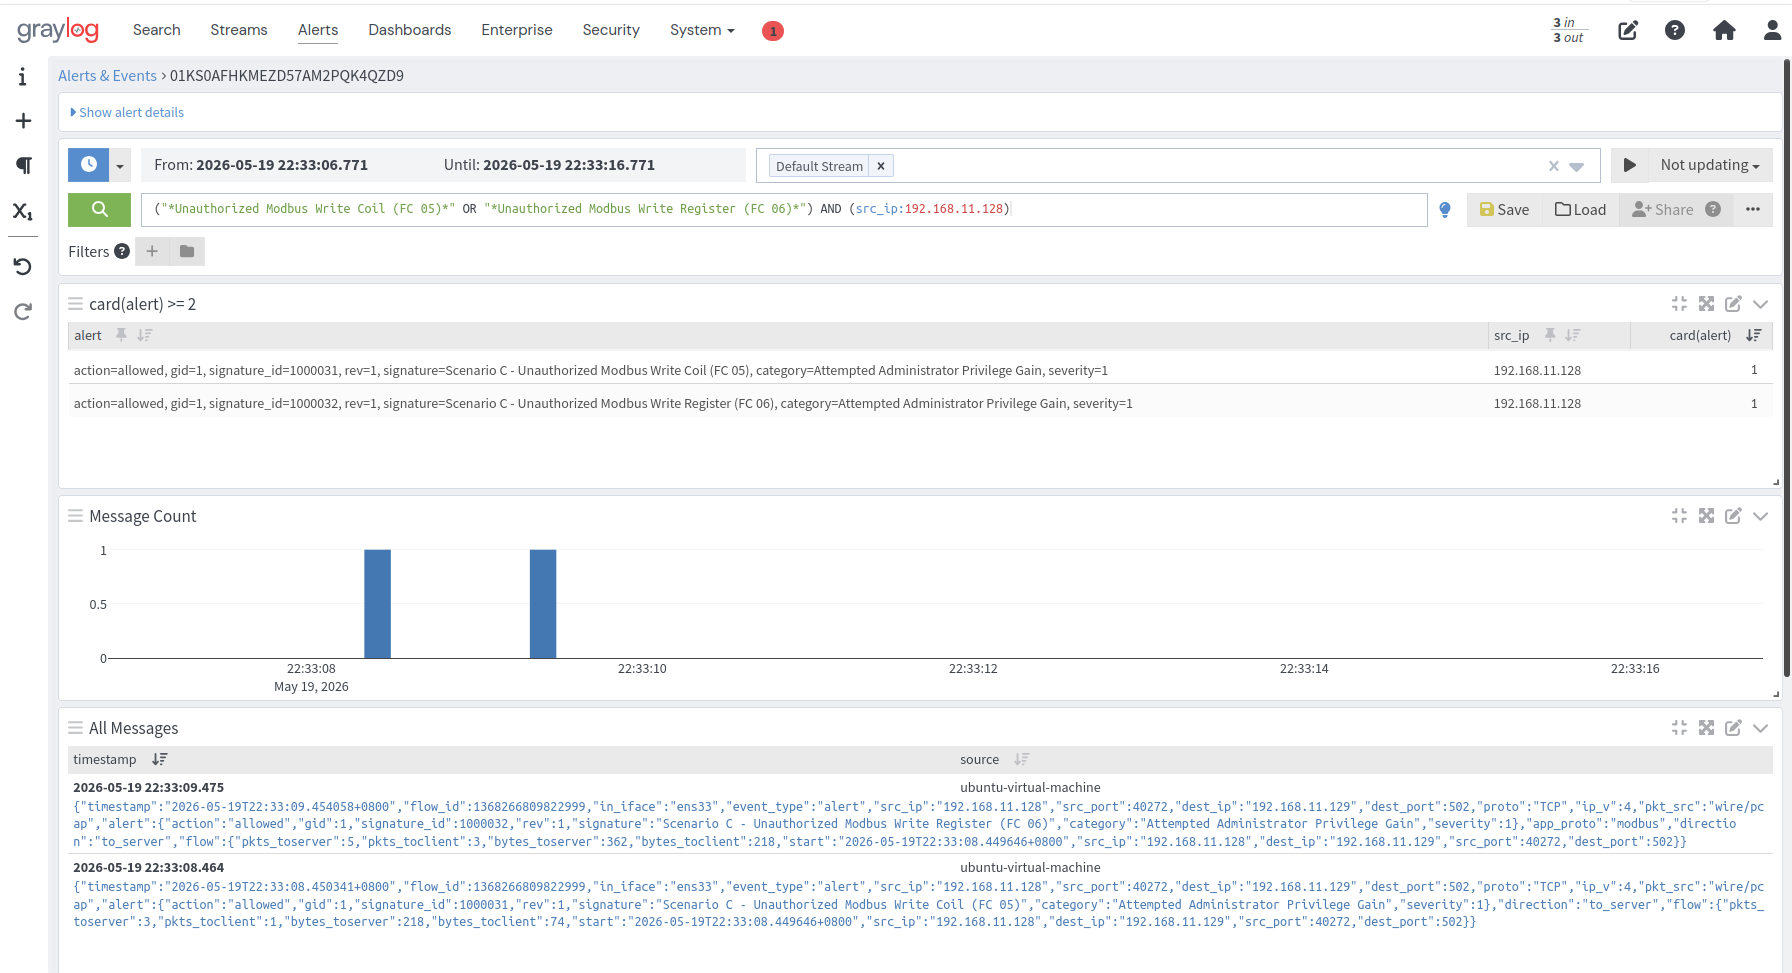
\includegraphics[width=0.9\textwidth]{figure/Figure_5.22.png}
    \caption{Graylog Dashboard for Modbus TCP Security Monitoring}
    \label{fig:Figure_5.22.png}
\end{figure}

In addition to visualization, Graylog notification mechanisms were used to support timely response. As illustrated in Figure~\ref{fig:Figure_5.23.png}, when a High severity event is generated, Graylog can trigger an instant notification to alert the operator. This mechanism is especially important for events such as unauthorized modification, critical command injection, and denial-of-service flooding because delayed response may affect system integrity or availability in OT environments.

\begin{figure}[H]
    \centering
    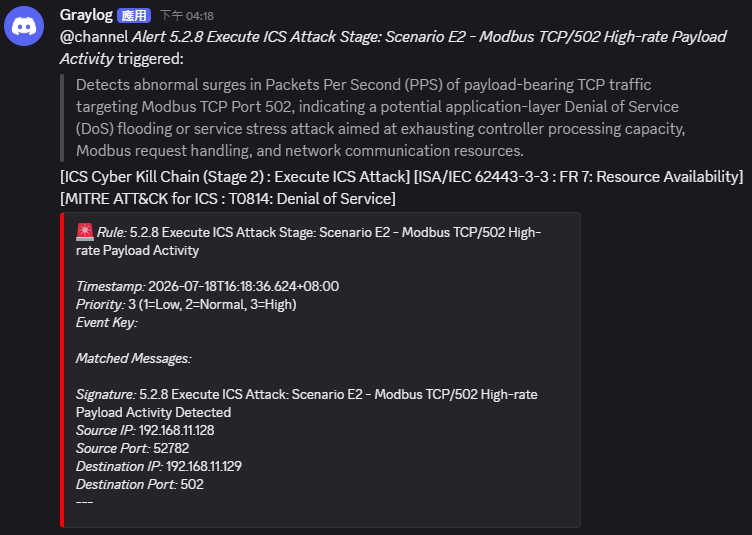
\includegraphics[width=0.75\textwidth]{figure/Figure_5.23.png}
    \caption{Graylog Instant Notification for High Severity Alert}
    \label{fig:Figure_5.23.png}
\end{figure}

\subsection{Traceability Summary}

The SIEM-based analysis improved event traceability in three aspects. First, each alert could be traced back to a specific Suricata rule and experimental scenario. Second, each event could be linked to communication context, including source IP, destination IP, destination port, Modbus function code, and event time. Third, each event could be mapped to ICS Cyber Kill Chain, ISA/IEC 62443-3-3, and MITRE ATT\&CK for ICS for attack-stage, security-requirement, and TTP-based interpretation.

Overall, the results show that the proposed framework not only detects Modbus TCP anomalies at the packet level, but also provides event-level correlation, traceability, visualization, and notification through SIEM integration.
\newpage
\section{Third-party Dataset and External Scenario Validation}

\subsection{Purpose and Validation Scope}
To avoid relying solely on the self-built experimental environment, this section further adopts third-party datasets and external attack-defense scenarios as supplementary validation sources. The main purpose of this third-party validation is to examine whether the scenario-based detection rules proposed in this research can be observed in Modbus TCP anomalies and attack indicators from different data sources. This helps evaluate the portability and applicability of the rules across different traffic environments.

It should be noted that the third-party validation in this section is positioned as supplementary validation, rather than a complete performance evaluation. This is because public datasets and external attack-defense scenarios usually do not provide the same asset roles, whitelist configurations, operating time windows, device address maps, or Graylog field structures as the self-built lab environment. Therefore, this section adopts a scenario-mapping approach to evaluate whether each rule's expected traffic conditions can be found in external data sources.

This validation complements the limitations of the self-built experimental environment. The lab validation in Section 5.2 provides controllability and reproducibility, confirming whether each rule can be correctly triggered under expected conditions. In contrast, the third-party validation in this section observes whether the corresponding traffic conditions exist in non-lab environments, thereby further supporting the external applicability of the proposed rule design.
\newpage

\subsection{Third-party Dataset Characteristics}
This research selects CICModbusDataset2023 and Modbus-related traffic from the 4SICS Geek Lounge as third-party validation sources. These two sources differ in data origin, traffic characteristics, and validation purpose. CICModbusDataset2023 is a relatively structured Modbus attack and anomaly dataset, making it suitable for comparing explicit protocol anomalies, write operations, and DoS-type behaviors. In contrast, the 4SICS Geek Lounge is closer to an attack-defense exercise or practical testing environment. Its traffic may contain more background traffic, scanning behavior, test packets, and non-fixed interaction patterns. Therefore, it is suitable for observing rule triggering in a less controlled environment.

Since the rules proposed in this research are mainly based on Modbus TCP protocol fields, Function Codes, Exception Responses, Diagnostic Sub-functions, and TCP/502 traffic rates, both external data sources can serve as references for evaluating rule portability. Table~\ref{tab:validation_data_sources} summarizes the differences in data characteristics among the two third-party sources and the self-built lab.

\begin{table}[htbp]
\caption{Characteristics of Validation Data Sources}
\centering
\footnotesize
\renewcommand{\arraystretch}{1.4}

\resizebox{\textwidth}{!}{%
\begin{tabular}{|>{\centering\arraybackslash}m{3.0cm}
                |>{\centering\arraybackslash}m{3.0cm}
                |>{\centering\arraybackslash}m{4.5cm}
                |>{\centering\arraybackslash}m{4.8cm}|}
\hline
\textbf{Data Source} & 
\textbf{Type} & 
\textbf{Main Purpose in This Research} & 
\textbf{Limitation} \\ 
\hline

Self-built Lab Testbed 
& Controlled experimental environment 
& Verifies whether each rule can be triggered under expected conditions. 
& May not fully represent external traffic diversity. \\ 
\hline

CICModbusDataset\newline2023
& Public structured Modbus dataset 
& Provides external reference for protocol anomalies, write operations, and DoS-like behavior. 
& Field labels, attack scripts, and environment settings may differ from this research. \\ 
\hline

4SICS Geek Lounge 
& External attack-defense / testbed traffic 
& Evaluates whether rules can be triggered in less controlled and more realistic traffic scenarios. 
& May lack complete ground truth, whitelist information, or consistent attack labels. \\ 
\hline

\end{tabular}%
}
\label{tab:validation_data_sources}
\end{table}
\newpage

\subsection{Validation Method and Mapping Criteria}
The third-party validation adopts a scenario-mapping approach. First, based on the rules defined in Chapter 4, this research summarizes the packet features and protocol conditions required for each scenario. These include FC17, FC43, unsupported Function Codes, the MBAP Protocol Identifier, Exception Codes, write-related Function Codes, FC08 sub-functions, TCP SYN rate, and payload-bearing packet rate. Second, the Modbus TCP packet features in third-party datasets or external traffic are compared with these conditions.

The third-party validation results are classified into two types: \textbf{Triggered} and \textbf{Not Observed}. Triggered indicates that the packet features or traffic conditions required by the rule are present in the data source, such that the rule can be triggered or the corresponding attack behavior can be confirmed. This includes cases where an alert is directly generated by Suricata or Graylog, as well as cases where the dataset itself explicitly labels the corresponding attack traffic that satisfies the rule condition. Not Observed indicates that no corresponding packet feature or behavior required by the rule is found in the data source, meaning the rule condition cannot be evaluated due to the absence of relevant traffic. The detailed definitions and examples of these two result types are summarized in Table~\ref{tab:mapping_criteria}.

\begin{table}[htbp]
\caption{Mapping Criteria for Third-party Validation}
\centering
\footnotesize
\renewcommand{\arraystretch}{1.4}

\resizebox{\textwidth}{!}{%
\begin{tabular}{|>{\bfseries\centering\arraybackslash}m{2.5cm}
                |>{\centering\arraybackslash}m{6.5cm}
                |>{\centering\arraybackslash}m{5.5cm}|}
\hline
\textbf{Result Type} & 
\textbf{Definition} & 
\textbf{Example} \\ 
\hline

Triggered 
& The packet features or traffic conditions required by the rule are present in the data source, either through a direct Suricata/Graylog alert or explicitly labeled attack traffic satisfying the rule condition. 
& Suricata generates an alert matching the corresponding SID; or the dataset contains FC05/FC06 write operations labeled as an attack. \\ 
\hline

Not Observed 
& No corresponding packet feature or behavior required by the rule is found in the data source, so the rule condition cannot be evaluated. 
& No FC08 diagnostic sub-function appears in the dataset. \\ 
\hline

\end{tabular}%
}
\label{tab:mapping_criteria}
\end{table}
\newpage

\subsection{External Scenario Mapping Results}
Table~\ref{tab:third_party_mapping} shows the mapping results of all scenario-based rules across the self-built lab, CICModbusDataset2023, and the 4SICS Geek Lounge. Overall, rules that depend on Exception Codes, write-related Function Codes, or traffic-rate thresholds, namely Response-side Modbus Exception Detection, Unauthorized Modification, and the two high-rate DoS-related scenarios, are Triggered across all three data sources. These rules mainly rely on packet fields or traffic-rate patterns that are commonly present regardless of the specific traffic environment.

In contrast, Reconnaissance Scanning, Request-side Modbus Protocol Probing, and Advanced Register Manipulation are Triggered in the self-built lab and the 4SICS Geek Lounge, but are Not Observed in CICModbusDataset2023. This is mainly because the CIC dataset does not contain device identification requests (FC17/FC43), unsupported Function Codes, or FC22/FC23 advanced register operations, rather than a limitation of the proposed rule design. Critical Diagnostic Command Injection remains the most environment-dependent scenario, as it is only Triggered in the self-built lab; both third-party sources lack FC08 diagnostic sub-function traffic, and therefore this scenario is Not Observed outside a controlled testbed.
\newpage
\begin{table}[htbp]
\caption{Third-party Dataset Mapping for Scenario-based Detection Rules}
\centering
\footnotesize
\renewcommand{\arraystretch}{1.5}

\resizebox{\textwidth}{!}{%
\begin{tabular}{|>{\bfseries\centering\arraybackslash}m{0.6cm}
                |>{\centering\arraybackslash}m{2.3cm}
                |>{\centering\arraybackslash}m{2.3cm}
                |>{\centering\arraybackslash}m{2.3cm}
                |>{\centering\arraybackslash}m{2.3cm}
                |>{\centering\arraybackslash}m{4.5cm}|}
\hline
\textbf{Rule ID} & 
\textbf{Scenario} & 
\textbf{CIC\newline ModbusDataset\newline2023} & 
\textbf{4SICS Geek Lounge} & 
\textbf{Ours} & 
\textbf{Mapping Basis} \\ 
\hline

A 
& Reconnaissance Scanning 
& Not Observed 
& Triggered 
& Triggered 
& Based on FC17, FC43, or device identification requests; not present in the CIC dataset traffic. \\ 
\hline

B1 
& Request-side Modbus Protocol Probing 
& Not Observed 
& Triggered 
& Triggered 
& Based on unsupported Function Codes or malformed MBAP headers; not present in the CIC dataset traffic. \\ 
\hline

B2 
& Response-side Modbus Exception  
& Triggered 
& Triggered 
& Triggered 
& Based on Exception Function Code and Exception Code. \\ 
\hline

C1 
& Unauthorized Modification 
& Triggered 
& Triggered 
& Triggered 
& Based on FC05, FC06, FC15, and FC16 write operations. \\ 
\hline

C2 
& Advanced Register Manipulation 
& Not Observed 
& Triggered 
& Triggered 
& Based on FC22 or FC23 advanced register operations; not present in the CIC dataset traffic. \\ 
\hline

D 
& Critical Diagnostic Command Injection 
& Not Observed 
& Not Observed 
& Triggered 
& Based on FC08 and specific diagnostic sub-functions; not present in either third-party source. \\ 
\hline

E1 
& High-rate SYN Activity 
& Triggered 
& Triggered 
& Triggered 
& Based on TCP/502 SYN packet rate and threshold. \\ 
\hline

E2 
& High-rate Payload Activity 
& Triggered 
& Triggered 
& Triggered 
& Based on TCP/502 payload-bearing packet rate and threshold. \\ 
\hline

\end{tabular}%
}
\label{tab:third_party_mapping}
\end{table}
\newpage
\section{System Performance and Latency Analysis}
To evaluate the operational feasibility of the proposed threat monitoring framework, we quantitatively analyzed both the end-to-end alerting latency across designed scenarios and the system's resource consumption under extreme traffic conditions. This quantitative evaluation defines the performance boundaries of our open-source passive detection pipeline.

\subsection{End-to-End Alerting Latency Evaluation}
In this evaluation, the end-to-end latency is defined as the elapsed time from the transmission of an adversarial packet from the attack host (VM1) to the successful reception of the corresponding severity alert on the operator's Slack client interface. This measurable latency is a cumulative result of several processing stages within the developed pipeline: (1) packet capture and deep packet inspection by Suricata at the interface layer; (2) JSON log generation and local syslog forwarding to the Graylog collector; (3) normalized field indexing, categorization, and correlation rule execution within Graylog; and (4) webhook execution and external network propagation to the Slack API. Table~\ref{tab:latency_measurements} presents the empirical measurements recorded over ten independent experimental runs for each threat scenario, along with the calculated mean latency for each column.

\begin{table}[H]
\centering
\caption{End-to-End Alerting Latency Measurements across Ten Experimental Runs (in Seconds).}
\label{tab:latency_measurements}
\begin{tabular}{ccccccccc}
\toprule
\textbf{Run No.} & \textbf{A} & \textbf{B1} & \textbf{B2} & \textbf{C1} & \textbf{C2} & \textbf{D} & \textbf{E1} & \textbf{E2} \\ \midrule
1 & 10.97 & 16.83 & 6.38 & 7.08 & 6.35 & 3.01 & 5.23 & 5.76 \\
2 & 6.05 & 6.13 & 7.25 & 6.67 & 6.47 & 4.91 & 8.08 & 4.55 \\
3 & 5.43 & 8.35 & 5.28 & 6.80 & 9.84 & 3.06 & 8.11 & 4.25 \\
4 & 7.32 & 12.34 & 3.95 & 10.27 & 5.80 & 7.57 & 15.53 & 7.96 \\
5 & 6.98 & 4.68 & 5.72 & 9.27 & 6.61 & 6.83 & 8.11 & 8.36 \\
6 & 6.52 & 4.23 & 5.03 & 3.80 & 8.58 & 2.60 & 4.98 & 8.31 \\
7 & 6.70 & 8.82 & 6.80 & 9.57 & 4.90 & 4.23 & 10.18 & 5.60 \\
8 & 5.15 & 8.77 & 5.13 & 3.58 & 5.30 & 5.33 & 8.48 & 7.46 \\
9 & 5.08 & 10.27 & 3.35 & 7.47 & 7.46 & 4.47 & 10.89 & 6.91 \\
10 & 5.23 & 9.84 & 7.83 & 8.67 & 9.01 & 6.70 & 15.95 & 6.33 \\ \midrule
\textbf{Mean} & \textbf{6.543} & \textbf{9.026} & \textbf{5.672} & \textbf{7.318} & \textbf{7.032} & \textbf{4.871} & \textbf{9.554} & \textbf{6.549} \\ \bottomrule
\end{tabular}
\end{table}
Based on the quantitative results, the average end-to-end alerting latency across all evaluated scenarios remains below 10 seconds. Variations in latency among the scenarios are directly attributable to the specific detection logic and processing requirements of each rule:
\begin{itemize}
    \item \textbf{Scenario D (Critical Diagnostic Command Injection):} Recorded the lowest mean latency of 4.871 seconds, because it matches against static, single-packet L7 payloads in Suricata (specific sub-functions of FC08), generating immediate alerts without requiring multi-event SIEM aggregation or stateful temporal analysis.
    \item \textbf{Scenario E1 (High-rate SYN Activity):} Exhibited the highest mean latency of 9.554 seconds, which is inherently influenced by the rate-based threshold configuration. To prevent false positives, the SIEM layer must aggregate TCP connection events over a defined sliding temporal window to verify whether the traffic volume crosses the threat threshold, thereby introducing an intentional aggregation delay.
    \item \textbf{Scenario B1 (Request-side Modbus Protocol Probing):} Recorded a mean latency of 9.026 seconds. Since B1 involves a sequence of alternating malformed packets and unsupported function codes generated by a fuzzing script, the Graylog correlation engine requires additional parsing cycles to aggregate the multi-packet stream and classify it as a single coherent scanning event.
\end{itemize}
\newpage
\subsection{System Stress and Resource Consumption Analysis}
To define the physical operational boundaries of the proposed framework, a high-rate stress test was executed within the virtualized lab environment over a continuous 300-second observation window. VM1 initiated a high-intensity TCP SYN flood attack targeting port 502 on VM2 using hping3 in flood mode, transmitting a total of 4,847,307 malicious packets, as shown in Figure~\ref{fig:Figure_5.24.png}. To quantitatively analyze the limits of our defensive pipeline under extreme load, network ingestion statistics on the interface card (ens33) and component-level resource consumption were logged at 1-second intervals.

\begin{figure}[H]
    \centering
    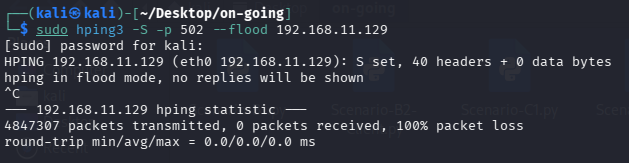
\includegraphics[width=0.9\textwidth]{figure/Figure_5.24.png}
    \caption{hping3 TCP SYN flood execution results showing the transmission of 4,847,307 malicious packets.}
    \label{fig:Figure_5.24.png}
\end{figure}

As detailed in Table~\ref{tab:stress_test_metrics} and visualized in Figure~\ref{fig:Figure_5.25.png}, the local network interface (\texttt{ens33}) maintained a sustained ingestion load, recording a mean packet rate of 18,751.89 PPS and peaking at 29,128.00 PPS. The network bandwidth utilization achieved a mean of 8.62 Mbps and peaked at 13.36 Mbps. These results highlight the small-frame nature of Modbus TCP traffic, where a massive frequency of command packets saturates processing pipelines without consuming substantial transmission bandwidth.
\begin{table}[H]
\centering
\caption{System Resource Consumption and Network Ingestion Performance under Peak Stress (300-Second Flood Window).}
\label{tab:stress_test_metrics}
\resizebox{\textwidth}{!}{%
\begin{tabular}{lccc}
\toprule
\textbf{Metric Type} & \textbf{Component / Interface} & \textbf{Average (Mean)} & \textbf{Peak (Maximum)} \\ \midrule
\textbf{Network Performance} & Packet Ingestion Rate (PPS) & 18,751.89 & 29,128.00 \\
& Ingestion Bandwidth (Mbps) & 8.62 & 13.36 \\ \midrule
\textbf{CPU Utilization (\%)} & Suricata DPI Engine & 36.45\% & 154.20\% \\
& Graylog SIEM Container & 36.28\% & 126.37\% \\
& OpenSearch DB Container & 16.08\% & 59.54\% \\
& MongoDB Store Container & 26.24\% & 81.73\% \\
& dockerd Host Service & 2.40\% & 61.90\% \\ \midrule
\textbf{Memory Utilization} & Graylog SIEM Container & 1.395 GiB (7.16\%) & 1.397 GiB (7.17\%) \\
& OpenSearch DB Container & 10.86 GiB (55.72\%) & 10.86 GiB (55.73\%) \\
& MongoDB Store Container & 139.9 MiB (0.70\%) & 140.2 MiB (0.70\%) \\ \midrule
\textbf{Data Integrity} & Suricata Socket Drop Rate (\%) & 0.00\% & 0.00\% \\
& Graylog Ingestion Loss Rate (\%) & 0.00\% & 0.00\% \\ \bottomrule
\end{tabular}%
}
\end{table}
\begin{figure}[H]
    \centering
    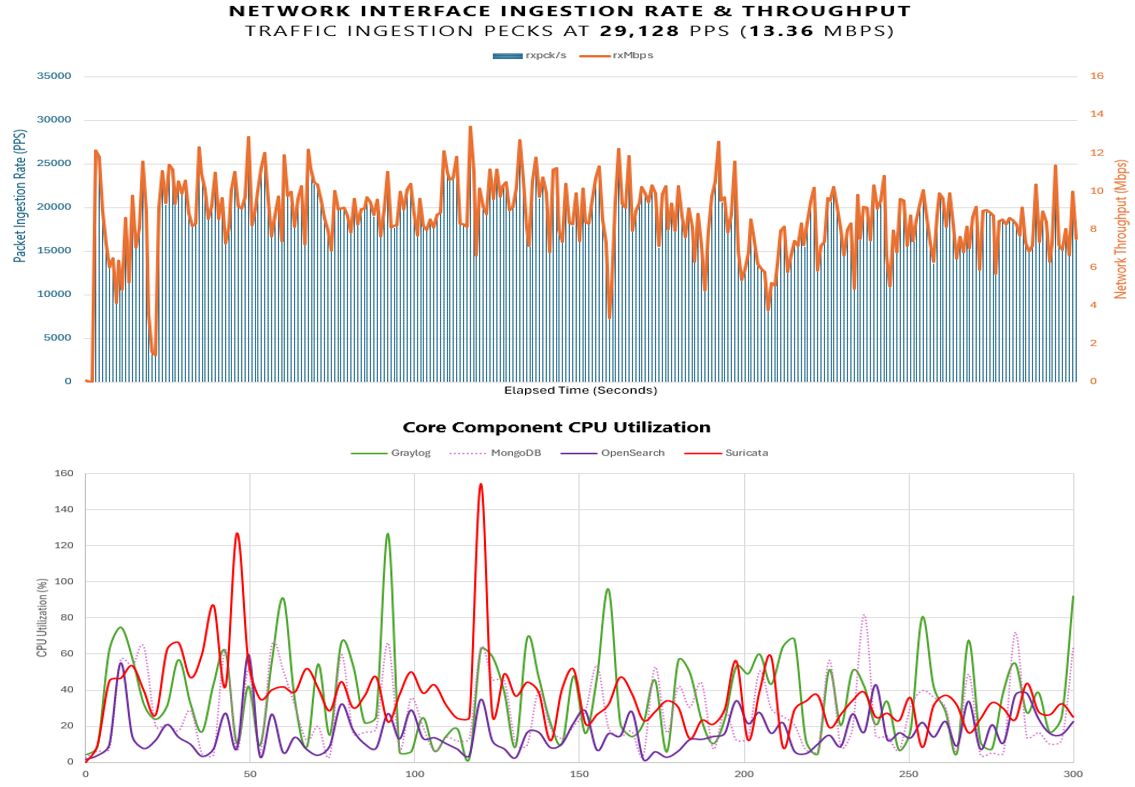
\includegraphics[width=0.9\textwidth]{figure/Figure_5.25.png}
    \caption{System stress-testing analysis over a 300-second flood window: \newline(a) network throughput, and (b) core component CPU utilization.}
    \label{fig:Figure_5.25.png}
\end{figure}
\newpage
Despite the intensive injection load, the system components demonstrated notable resource stability and operational safety margins:
\begin{itemize}
    \item \textbf{Suricata DPI Layer:} The rule-based Suricata engine consumed a mean CPU of 36.45\% and peaked at 154.20\%. Because the peak CPU consumption remained well within the limits of the allocated 4 vCPUs, the engine achieved a 0.00\% kernel socket packet drop rate (\texttt{capture.kernel\_drops = 0}), ensuring that no captured traffic bypassed the deep packet inspection layer.
    \item \textbf{SIEM Container Pipeline:} Graylog and its supporting databases (OpenSearch and MongoDB) demonstrated highly stable memory profiles throughout the flood. OpenSearch maintained a flat memory footprint of approximately 10.86 GiB (55.72\%) to support the database's write indexing, while Graylog's memory utilization remained constant at 1.395 GiB (7.16\%). Under peak traffic processing, Graylog's CPU utilization peaked at 126.37\% with a mean of 36.28\%, and MongoDB peaked at 81.73\% with a mean of 26.24\%.
\end{itemize}

Throughout the entire process, no log loss or database write errors (0.00\% log drop rate) were detected within the SIEM layer. These quantitative results confirm that deploying the proposed open-source monitoring framework on lightweight, low-cost virtualized hardware does not introduce defensive blind spots or data loss risks during security incidents, thereby demonstrating exceptional practical feasibility for real-world deployment.
\newpage
\section{Discussion and Limitations}
The third-party validation results show that the scenario-based rules proposed in this research have a certain degree of external applicability, although the extent to which each rule is Triggered varies across data sources. Rules centered on Exception Codes, write-related Function Codes, and traffic-rate thresholds, namely Response-side Exception Detection, Unauthorized Modification, and the two high-rate DoS scenarios, are consistently Triggered across the self-built lab, the 4SICS Geek Lounge, and CICModbusDataset2023. This indicates that the proposed rule design is not limited to the self-built lab environment and has a certain degree of portability for these scenarios.

However, the results in this section also reveal several limitations of third-party validation, domain context, and passive architecture.

\subsection{Domain Knowledge Dependency in ICS Environments}
A major limitation of rule-based OT security monitoring lies in the heavy dependency on site-specific domain knowledge. While the proposed Unauthorized Modification rules can successfully flag write commands (such as FC05, FC06, FC15, or FC16) originating from non-whitelisted source IPs, evaluating whether the specific values written to the registers are operationally safe remains an open challenge. 

For instance, a register write command modifying a temperature or motor speed setpoint via FC06 might carry a perfectly benign value for one production line but represent a catastrophic setting for another. Because different industrial facilities operate under completely unique physical parameters and control loops, determining the semantic legitimacy of register payloads inherently requires deep integration with the specific factory's process engineering domain knowledge, which cannot be easily generalized using static, signature-based rules.

\subsection{Vulnerabilities of Passive Sniffing and Intra-subnet Attacks}
Another critical limitation stems from the passive monitoring architecture and the physical topology of OT networks. Although passive network sniffing ensures zero interference with real-time OT communications—complying with the high-availability requirements of industrial networks—it introduces defensive blind spots against sophisticated intra-subnet attacks. 

Because the Suricata DPI engine operates out-of-band and does not act as an inline gateway, it cannot actively intercept or block transit traffic. Consequently, if an adversary already lurking within the same local subnet executes spoofing attacks (e.g., ARP poisoning or IP spoofing) to impersonate a trusted HMI, or actively injects malicious TCP connection teardowns (such as RST floods) to disrupt PLC communications, the passive system can only log and alert retrospectively. It lacks the active control capability to physically disrupt such attacks before physical process impact occurs.

Therefore, this research treats third-party dataset validation as supplementary evidence to support the applicability of the rules across different traffic sources, rather than as a replacement for the controlled and reproducible lab validation. In future deployment of this framework, standardized field transformation processes, asset role labeling, and threshold calibration methods can be further established for third-party datasets to quantitatively evaluate the detection performance of each rule across different data sources.


